\documentclass[11pt]{article}

    \usepackage[breakable]{tcolorbox}
    \usepackage{parskip} % Stop auto-indenting (to mimic markdown behaviour)
    
    \usepackage{iftex}
    \ifPDFTeX
    	\usepackage[T1]{fontenc}
    	\usepackage{mathpazo}
    \else
    	\usepackage{fontspec}
    \fi

    % Basic figure setup, for now with no caption control since it's done
    % automatically by Pandoc (which extracts ![](path) syntax from Markdown).
    \usepackage{graphicx}
    % Maintain compatibility with old templates. Remove in nbconvert 6.0
    \let\Oldincludegraphics\includegraphics
    % Ensure that by default, figures have no caption (until we provide a
    % proper Figure object with a Caption API and a way to capture that
    % in the conversion process - todo).
    \usepackage{caption}
    \DeclareCaptionFormat{nocaption}{}
    \captionsetup{format=nocaption,aboveskip=0pt,belowskip=0pt}

    \usepackage[Export]{adjustbox} % Used to constrain images to a maximum size
    \adjustboxset{max size={0.9\linewidth}{0.9\paperheight}}
    \usepackage{float}
    \floatplacement{figure}{H} % forces figures to be placed at the correct location
    \usepackage{xcolor} % Allow colors to be defined
    \usepackage{enumerate} % Needed for markdown enumerations to work
    \usepackage{geometry} % Used to adjust the document margins
    \usepackage{amsmath} % Equations
    \usepackage{amssymb} % Equations
    \usepackage{textcomp} % defines textquotesingle
    % Hack from http://tex.stackexchange.com/a/47451/13684:
    \AtBeginDocument{%
        \def\PYZsq{\textquotesingle}% Upright quotes in Pygmentized code
    }
    \usepackage{upquote} % Upright quotes for verbatim code
    \usepackage{eurosym} % defines \euro
    \usepackage[mathletters]{ucs} % Extended unicode (utf-8) support
    \usepackage{fancyvrb} % verbatim replacement that allows latex
    \usepackage{grffile} % extends the file name processing of package graphics 
                         % to support a larger range
    \makeatletter % fix for grffile with XeLaTeX
    \def\Gread@@xetex#1{%
      \IfFileExists{"\Gin@base".bb}%
      {\Gread@eps{\Gin@base.bb}}%
      {\Gread@@xetex@aux#1}%
    }
    \makeatother

    % The hyperref package gives us a pdf with properly built
    % internal navigation ('pdf bookmarks' for the table of contents,
    % internal cross-reference links, web links for URLs, etc.)
    \usepackage{hyperref}
    % The default LaTeX title has an obnoxious amount of whitespace. By default,
    % titling removes some of it. It also provides customization options.
    \usepackage{titling}
    \usepackage{longtable} % longtable support required by pandoc >1.10
    \usepackage{booktabs}  % table support for pandoc > 1.12.2
    \usepackage[inline]{enumitem} % IRkernel/repr support (it uses the enumerate* environment)
    \usepackage[normalem]{ulem} % ulem is needed to support strikethroughs (\sout)
                                % normalem makes italics be italics, not underlines
    \usepackage{mathrsfs}
    

    
    % Colors for the hyperref package
    \definecolor{urlcolor}{rgb}{0,.145,.698}
    \definecolor{linkcolor}{rgb}{.71,0.21,0.01}
    \definecolor{citecolor}{rgb}{.12,.54,.11}

    % ANSI colors
    \definecolor{ansi-black}{HTML}{3E424D}
    \definecolor{ansi-black-intense}{HTML}{282C36}
    \definecolor{ansi-red}{HTML}{E75C58}
    \definecolor{ansi-red-intense}{HTML}{B22B31}
    \definecolor{ansi-green}{HTML}{00A250}
    \definecolor{ansi-green-intense}{HTML}{007427}
    \definecolor{ansi-yellow}{HTML}{DDB62B}
    \definecolor{ansi-yellow-intense}{HTML}{B27D12}
    \definecolor{ansi-blue}{HTML}{208FFB}
    \definecolor{ansi-blue-intense}{HTML}{0065CA}
    \definecolor{ansi-magenta}{HTML}{D160C4}
    \definecolor{ansi-magenta-intense}{HTML}{A03196}
    \definecolor{ansi-cyan}{HTML}{60C6C8}
    \definecolor{ansi-cyan-intense}{HTML}{258F8F}
    \definecolor{ansi-white}{HTML}{C5C1B4}
    \definecolor{ansi-white-intense}{HTML}{A1A6B2}
    \definecolor{ansi-default-inverse-fg}{HTML}{FFFFFF}
    \definecolor{ansi-default-inverse-bg}{HTML}{000000}

    % commands and environments needed by pandoc snippets
    % extracted from the output of `pandoc -s`
    \providecommand{\tightlist}{%
      \setlength{\itemsep}{0pt}\setlength{\parskip}{0pt}}
    \DefineVerbatimEnvironment{Highlighting}{Verbatim}{commandchars=\\\{\}}
    % Add ',fontsize=\small' for more characters per line
    \newenvironment{Shaded}{}{}
    \newcommand{\KeywordTok}[1]{\textcolor[rgb]{0.00,0.44,0.13}{\textbf{{#1}}}}
    \newcommand{\DataTypeTok}[1]{\textcolor[rgb]{0.56,0.13,0.00}{{#1}}}
    \newcommand{\DecValTok}[1]{\textcolor[rgb]{0.25,0.63,0.44}{{#1}}}
    \newcommand{\BaseNTok}[1]{\textcolor[rgb]{0.25,0.63,0.44}{{#1}}}
    \newcommand{\FloatTok}[1]{\textcolor[rgb]{0.25,0.63,0.44}{{#1}}}
    \newcommand{\CharTok}[1]{\textcolor[rgb]{0.25,0.44,0.63}{{#1}}}
    \newcommand{\StringTok}[1]{\textcolor[rgb]{0.25,0.44,0.63}{{#1}}}
    \newcommand{\CommentTok}[1]{\textcolor[rgb]{0.38,0.63,0.69}{\textit{{#1}}}}
    \newcommand{\OtherTok}[1]{\textcolor[rgb]{0.00,0.44,0.13}{{#1}}}
    \newcommand{\AlertTok}[1]{\textcolor[rgb]{1.00,0.00,0.00}{\textbf{{#1}}}}
    \newcommand{\FunctionTok}[1]{\textcolor[rgb]{0.02,0.16,0.49}{{#1}}}
    \newcommand{\RegionMarkerTok}[1]{{#1}}
    \newcommand{\ErrorTok}[1]{\textcolor[rgb]{1.00,0.00,0.00}{\textbf{{#1}}}}
    \newcommand{\NormalTok}[1]{{#1}}
    
    % Additional commands for more recent versions of Pandoc
    \newcommand{\ConstantTok}[1]{\textcolor[rgb]{0.53,0.00,0.00}{{#1}}}
    \newcommand{\SpecialCharTok}[1]{\textcolor[rgb]{0.25,0.44,0.63}{{#1}}}
    \newcommand{\VerbatimStringTok}[1]{\textcolor[rgb]{0.25,0.44,0.63}{{#1}}}
    \newcommand{\SpecialStringTok}[1]{\textcolor[rgb]{0.73,0.40,0.53}{{#1}}}
    \newcommand{\ImportTok}[1]{{#1}}
    \newcommand{\DocumentationTok}[1]{\textcolor[rgb]{0.73,0.13,0.13}{\textit{{#1}}}}
    \newcommand{\AnnotationTok}[1]{\textcolor[rgb]{0.38,0.63,0.69}{\textbf{\textit{{#1}}}}}
    \newcommand{\CommentVarTok}[1]{\textcolor[rgb]{0.38,0.63,0.69}{\textbf{\textit{{#1}}}}}
    \newcommand{\VariableTok}[1]{\textcolor[rgb]{0.10,0.09,0.49}{{#1}}}
    \newcommand{\ControlFlowTok}[1]{\textcolor[rgb]{0.00,0.44,0.13}{\textbf{{#1}}}}
    \newcommand{\OperatorTok}[1]{\textcolor[rgb]{0.40,0.40,0.40}{{#1}}}
    \newcommand{\BuiltInTok}[1]{{#1}}
    \newcommand{\ExtensionTok}[1]{{#1}}
    \newcommand{\PreprocessorTok}[1]{\textcolor[rgb]{0.74,0.48,0.00}{{#1}}}
    \newcommand{\AttributeTok}[1]{\textcolor[rgb]{0.49,0.56,0.16}{{#1}}}
    \newcommand{\InformationTok}[1]{\textcolor[rgb]{0.38,0.63,0.69}{\textbf{\textit{{#1}}}}}
    \newcommand{\WarningTok}[1]{\textcolor[rgb]{0.38,0.63,0.69}{\textbf{\textit{{#1}}}}}
    
    
    % Define a nice break command that doesn't care if a line doesn't already
    % exist.
    \def\br{\hspace*{\fill} \\* }
    % Math Jax compatibility definitions
    \def\gt{>}
    \def\lt{<}
    \let\Oldtex\TeX
    \let\Oldlatex\LaTeX
    \renewcommand{\TeX}{\textrm{\Oldtex}}
    \renewcommand{\LaTeX}{\textrm{\Oldlatex}}
    % Document parameters
    % Document title
    \title{12-PySpark}
    
    
    
    \author{Pierre Navaro}
    
    
    
% Pygments definitions
\makeatletter
\def\PY@reset{\let\PY@it=\relax \let\PY@bf=\relax%
    \let\PY@ul=\relax \let\PY@tc=\relax%
    \let\PY@bc=\relax \let\PY@ff=\relax}
\def\PY@tok#1{\csname PY@tok@#1\endcsname}
\def\PY@toks#1+{\ifx\relax#1\empty\else%
    \PY@tok{#1}\expandafter\PY@toks\fi}
\def\PY@do#1{\PY@bc{\PY@tc{\PY@ul{%
    \PY@it{\PY@bf{\PY@ff{#1}}}}}}}
\def\PY#1#2{\PY@reset\PY@toks#1+\relax+\PY@do{#2}}

\expandafter\def\csname PY@tok@w\endcsname{\def\PY@tc##1{\textcolor[rgb]{0.73,0.73,0.73}{##1}}}
\expandafter\def\csname PY@tok@c\endcsname{\let\PY@it=\textit\def\PY@tc##1{\textcolor[rgb]{0.25,0.50,0.50}{##1}}}
\expandafter\def\csname PY@tok@cp\endcsname{\def\PY@tc##1{\textcolor[rgb]{0.74,0.48,0.00}{##1}}}
\expandafter\def\csname PY@tok@k\endcsname{\let\PY@bf=\textbf\def\PY@tc##1{\textcolor[rgb]{0.00,0.50,0.00}{##1}}}
\expandafter\def\csname PY@tok@kp\endcsname{\def\PY@tc##1{\textcolor[rgb]{0.00,0.50,0.00}{##1}}}
\expandafter\def\csname PY@tok@kt\endcsname{\def\PY@tc##1{\textcolor[rgb]{0.69,0.00,0.25}{##1}}}
\expandafter\def\csname PY@tok@o\endcsname{\def\PY@tc##1{\textcolor[rgb]{0.40,0.40,0.40}{##1}}}
\expandafter\def\csname PY@tok@ow\endcsname{\let\PY@bf=\textbf\def\PY@tc##1{\textcolor[rgb]{0.67,0.13,1.00}{##1}}}
\expandafter\def\csname PY@tok@nb\endcsname{\def\PY@tc##1{\textcolor[rgb]{0.00,0.50,0.00}{##1}}}
\expandafter\def\csname PY@tok@nf\endcsname{\def\PY@tc##1{\textcolor[rgb]{0.00,0.00,1.00}{##1}}}
\expandafter\def\csname PY@tok@nc\endcsname{\let\PY@bf=\textbf\def\PY@tc##1{\textcolor[rgb]{0.00,0.00,1.00}{##1}}}
\expandafter\def\csname PY@tok@nn\endcsname{\let\PY@bf=\textbf\def\PY@tc##1{\textcolor[rgb]{0.00,0.00,1.00}{##1}}}
\expandafter\def\csname PY@tok@ne\endcsname{\let\PY@bf=\textbf\def\PY@tc##1{\textcolor[rgb]{0.82,0.25,0.23}{##1}}}
\expandafter\def\csname PY@tok@nv\endcsname{\def\PY@tc##1{\textcolor[rgb]{0.10,0.09,0.49}{##1}}}
\expandafter\def\csname PY@tok@no\endcsname{\def\PY@tc##1{\textcolor[rgb]{0.53,0.00,0.00}{##1}}}
\expandafter\def\csname PY@tok@nl\endcsname{\def\PY@tc##1{\textcolor[rgb]{0.63,0.63,0.00}{##1}}}
\expandafter\def\csname PY@tok@ni\endcsname{\let\PY@bf=\textbf\def\PY@tc##1{\textcolor[rgb]{0.60,0.60,0.60}{##1}}}
\expandafter\def\csname PY@tok@na\endcsname{\def\PY@tc##1{\textcolor[rgb]{0.49,0.56,0.16}{##1}}}
\expandafter\def\csname PY@tok@nt\endcsname{\let\PY@bf=\textbf\def\PY@tc##1{\textcolor[rgb]{0.00,0.50,0.00}{##1}}}
\expandafter\def\csname PY@tok@nd\endcsname{\def\PY@tc##1{\textcolor[rgb]{0.67,0.13,1.00}{##1}}}
\expandafter\def\csname PY@tok@s\endcsname{\def\PY@tc##1{\textcolor[rgb]{0.73,0.13,0.13}{##1}}}
\expandafter\def\csname PY@tok@sd\endcsname{\let\PY@it=\textit\def\PY@tc##1{\textcolor[rgb]{0.73,0.13,0.13}{##1}}}
\expandafter\def\csname PY@tok@si\endcsname{\let\PY@bf=\textbf\def\PY@tc##1{\textcolor[rgb]{0.73,0.40,0.53}{##1}}}
\expandafter\def\csname PY@tok@se\endcsname{\let\PY@bf=\textbf\def\PY@tc##1{\textcolor[rgb]{0.73,0.40,0.13}{##1}}}
\expandafter\def\csname PY@tok@sr\endcsname{\def\PY@tc##1{\textcolor[rgb]{0.73,0.40,0.53}{##1}}}
\expandafter\def\csname PY@tok@ss\endcsname{\def\PY@tc##1{\textcolor[rgb]{0.10,0.09,0.49}{##1}}}
\expandafter\def\csname PY@tok@sx\endcsname{\def\PY@tc##1{\textcolor[rgb]{0.00,0.50,0.00}{##1}}}
\expandafter\def\csname PY@tok@m\endcsname{\def\PY@tc##1{\textcolor[rgb]{0.40,0.40,0.40}{##1}}}
\expandafter\def\csname PY@tok@gh\endcsname{\let\PY@bf=\textbf\def\PY@tc##1{\textcolor[rgb]{0.00,0.00,0.50}{##1}}}
\expandafter\def\csname PY@tok@gu\endcsname{\let\PY@bf=\textbf\def\PY@tc##1{\textcolor[rgb]{0.50,0.00,0.50}{##1}}}
\expandafter\def\csname PY@tok@gd\endcsname{\def\PY@tc##1{\textcolor[rgb]{0.63,0.00,0.00}{##1}}}
\expandafter\def\csname PY@tok@gi\endcsname{\def\PY@tc##1{\textcolor[rgb]{0.00,0.63,0.00}{##1}}}
\expandafter\def\csname PY@tok@gr\endcsname{\def\PY@tc##1{\textcolor[rgb]{1.00,0.00,0.00}{##1}}}
\expandafter\def\csname PY@tok@ge\endcsname{\let\PY@it=\textit}
\expandafter\def\csname PY@tok@gs\endcsname{\let\PY@bf=\textbf}
\expandafter\def\csname PY@tok@gp\endcsname{\let\PY@bf=\textbf\def\PY@tc##1{\textcolor[rgb]{0.00,0.00,0.50}{##1}}}
\expandafter\def\csname PY@tok@go\endcsname{\def\PY@tc##1{\textcolor[rgb]{0.53,0.53,0.53}{##1}}}
\expandafter\def\csname PY@tok@gt\endcsname{\def\PY@tc##1{\textcolor[rgb]{0.00,0.27,0.87}{##1}}}
\expandafter\def\csname PY@tok@err\endcsname{\def\PY@bc##1{\setlength{\fboxsep}{0pt}\fcolorbox[rgb]{1.00,0.00,0.00}{1,1,1}{\strut ##1}}}
\expandafter\def\csname PY@tok@kc\endcsname{\let\PY@bf=\textbf\def\PY@tc##1{\textcolor[rgb]{0.00,0.50,0.00}{##1}}}
\expandafter\def\csname PY@tok@kd\endcsname{\let\PY@bf=\textbf\def\PY@tc##1{\textcolor[rgb]{0.00,0.50,0.00}{##1}}}
\expandafter\def\csname PY@tok@kn\endcsname{\let\PY@bf=\textbf\def\PY@tc##1{\textcolor[rgb]{0.00,0.50,0.00}{##1}}}
\expandafter\def\csname PY@tok@kr\endcsname{\let\PY@bf=\textbf\def\PY@tc##1{\textcolor[rgb]{0.00,0.50,0.00}{##1}}}
\expandafter\def\csname PY@tok@bp\endcsname{\def\PY@tc##1{\textcolor[rgb]{0.00,0.50,0.00}{##1}}}
\expandafter\def\csname PY@tok@fm\endcsname{\def\PY@tc##1{\textcolor[rgb]{0.00,0.00,1.00}{##1}}}
\expandafter\def\csname PY@tok@vc\endcsname{\def\PY@tc##1{\textcolor[rgb]{0.10,0.09,0.49}{##1}}}
\expandafter\def\csname PY@tok@vg\endcsname{\def\PY@tc##1{\textcolor[rgb]{0.10,0.09,0.49}{##1}}}
\expandafter\def\csname PY@tok@vi\endcsname{\def\PY@tc##1{\textcolor[rgb]{0.10,0.09,0.49}{##1}}}
\expandafter\def\csname PY@tok@vm\endcsname{\def\PY@tc##1{\textcolor[rgb]{0.10,0.09,0.49}{##1}}}
\expandafter\def\csname PY@tok@sa\endcsname{\def\PY@tc##1{\textcolor[rgb]{0.73,0.13,0.13}{##1}}}
\expandafter\def\csname PY@tok@sb\endcsname{\def\PY@tc##1{\textcolor[rgb]{0.73,0.13,0.13}{##1}}}
\expandafter\def\csname PY@tok@sc\endcsname{\def\PY@tc##1{\textcolor[rgb]{0.73,0.13,0.13}{##1}}}
\expandafter\def\csname PY@tok@dl\endcsname{\def\PY@tc##1{\textcolor[rgb]{0.73,0.13,0.13}{##1}}}
\expandafter\def\csname PY@tok@s2\endcsname{\def\PY@tc##1{\textcolor[rgb]{0.73,0.13,0.13}{##1}}}
\expandafter\def\csname PY@tok@sh\endcsname{\def\PY@tc##1{\textcolor[rgb]{0.73,0.13,0.13}{##1}}}
\expandafter\def\csname PY@tok@s1\endcsname{\def\PY@tc##1{\textcolor[rgb]{0.73,0.13,0.13}{##1}}}
\expandafter\def\csname PY@tok@mb\endcsname{\def\PY@tc##1{\textcolor[rgb]{0.40,0.40,0.40}{##1}}}
\expandafter\def\csname PY@tok@mf\endcsname{\def\PY@tc##1{\textcolor[rgb]{0.40,0.40,0.40}{##1}}}
\expandafter\def\csname PY@tok@mh\endcsname{\def\PY@tc##1{\textcolor[rgb]{0.40,0.40,0.40}{##1}}}
\expandafter\def\csname PY@tok@mi\endcsname{\def\PY@tc##1{\textcolor[rgb]{0.40,0.40,0.40}{##1}}}
\expandafter\def\csname PY@tok@il\endcsname{\def\PY@tc##1{\textcolor[rgb]{0.40,0.40,0.40}{##1}}}
\expandafter\def\csname PY@tok@mo\endcsname{\def\PY@tc##1{\textcolor[rgb]{0.40,0.40,0.40}{##1}}}
\expandafter\def\csname PY@tok@ch\endcsname{\let\PY@it=\textit\def\PY@tc##1{\textcolor[rgb]{0.25,0.50,0.50}{##1}}}
\expandafter\def\csname PY@tok@cm\endcsname{\let\PY@it=\textit\def\PY@tc##1{\textcolor[rgb]{0.25,0.50,0.50}{##1}}}
\expandafter\def\csname PY@tok@cpf\endcsname{\let\PY@it=\textit\def\PY@tc##1{\textcolor[rgb]{0.25,0.50,0.50}{##1}}}
\expandafter\def\csname PY@tok@c1\endcsname{\let\PY@it=\textit\def\PY@tc##1{\textcolor[rgb]{0.25,0.50,0.50}{##1}}}
\expandafter\def\csname PY@tok@cs\endcsname{\let\PY@it=\textit\def\PY@tc##1{\textcolor[rgb]{0.25,0.50,0.50}{##1}}}

\def\PYZbs{\char`\\}
\def\PYZus{\char`\_}
\def\PYZob{\char`\{}
\def\PYZcb{\char`\}}
\def\PYZca{\char`\^}
\def\PYZam{\char`\&}
\def\PYZlt{\char`\<}
\def\PYZgt{\char`\>}
\def\PYZsh{\char`\#}
\def\PYZpc{\char`\%}
\def\PYZdl{\char`\$}
\def\PYZhy{\char`\-}
\def\PYZsq{\char`\'}
\def\PYZdq{\char`\"}
\def\PYZti{\char`\~}
% for compatibility with earlier versions
\def\PYZat{@}
\def\PYZlb{[}
\def\PYZrb{]}
\makeatother


    % For linebreaks inside Verbatim environment from package fancyvrb. 
    \makeatletter
        \newbox\Wrappedcontinuationbox 
        \newbox\Wrappedvisiblespacebox 
        \newcommand*\Wrappedvisiblespace {\textcolor{red}{\textvisiblespace}} 
        \newcommand*\Wrappedcontinuationsymbol {\textcolor{red}{\llap{\tiny$\m@th\hookrightarrow$}}} 
        \newcommand*\Wrappedcontinuationindent {3ex } 
        \newcommand*\Wrappedafterbreak {\kern\Wrappedcontinuationindent\copy\Wrappedcontinuationbox} 
        % Take advantage of the already applied Pygments mark-up to insert 
        % potential linebreaks for TeX processing. 
        %        {, <, #, %, $, ' and ": go to next line. 
        %        _, }, ^, &, >, - and ~: stay at end of broken line. 
        % Use of \textquotesingle for straight quote. 
        \newcommand*\Wrappedbreaksatspecials {% 
            \def\PYGZus{\discretionary{\char`\_}{\Wrappedafterbreak}{\char`\_}}% 
            \def\PYGZob{\discretionary{}{\Wrappedafterbreak\char`\{}{\char`\{}}% 
            \def\PYGZcb{\discretionary{\char`\}}{\Wrappedafterbreak}{\char`\}}}% 
            \def\PYGZca{\discretionary{\char`\^}{\Wrappedafterbreak}{\char`\^}}% 
            \def\PYGZam{\discretionary{\char`\&}{\Wrappedafterbreak}{\char`\&}}% 
            \def\PYGZlt{\discretionary{}{\Wrappedafterbreak\char`\<}{\char`\<}}% 
            \def\PYGZgt{\discretionary{\char`\>}{\Wrappedafterbreak}{\char`\>}}% 
            \def\PYGZsh{\discretionary{}{\Wrappedafterbreak\char`\#}{\char`\#}}% 
            \def\PYGZpc{\discretionary{}{\Wrappedafterbreak\char`\%}{\char`\%}}% 
            \def\PYGZdl{\discretionary{}{\Wrappedafterbreak\char`\$}{\char`\$}}% 
            \def\PYGZhy{\discretionary{\char`\-}{\Wrappedafterbreak}{\char`\-}}% 
            \def\PYGZsq{\discretionary{}{\Wrappedafterbreak\textquotesingle}{\textquotesingle}}% 
            \def\PYGZdq{\discretionary{}{\Wrappedafterbreak\char`\"}{\char`\"}}% 
            \def\PYGZti{\discretionary{\char`\~}{\Wrappedafterbreak}{\char`\~}}% 
        } 
        % Some characters . , ; ? ! / are not pygmentized. 
        % This macro makes them "active" and they will insert potential linebreaks 
        \newcommand*\Wrappedbreaksatpunct {% 
            \lccode`\~`\.\lowercase{\def~}{\discretionary{\hbox{\char`\.}}{\Wrappedafterbreak}{\hbox{\char`\.}}}% 
            \lccode`\~`\,\lowercase{\def~}{\discretionary{\hbox{\char`\,}}{\Wrappedafterbreak}{\hbox{\char`\,}}}% 
            \lccode`\~`\;\lowercase{\def~}{\discretionary{\hbox{\char`\;}}{\Wrappedafterbreak}{\hbox{\char`\;}}}% 
            \lccode`\~`\:\lowercase{\def~}{\discretionary{\hbox{\char`\:}}{\Wrappedafterbreak}{\hbox{\char`\:}}}% 
            \lccode`\~`\?\lowercase{\def~}{\discretionary{\hbox{\char`\?}}{\Wrappedafterbreak}{\hbox{\char`\?}}}% 
            \lccode`\~`\!\lowercase{\def~}{\discretionary{\hbox{\char`\!}}{\Wrappedafterbreak}{\hbox{\char`\!}}}% 
            \lccode`\~`\/\lowercase{\def~}{\discretionary{\hbox{\char`\/}}{\Wrappedafterbreak}{\hbox{\char`\/}}}% 
            \catcode`\.\active
            \catcode`\,\active 
            \catcode`\;\active
            \catcode`\:\active
            \catcode`\?\active
            \catcode`\!\active
            \catcode`\/\active 
            \lccode`\~`\~ 	
        }
    \makeatother

    \let\OriginalVerbatim=\Verbatim
    \makeatletter
    \renewcommand{\Verbatim}[1][1]{%
        %\parskip\z@skip
        \sbox\Wrappedcontinuationbox {\Wrappedcontinuationsymbol}%
        \sbox\Wrappedvisiblespacebox {\FV@SetupFont\Wrappedvisiblespace}%
        \def\FancyVerbFormatLine ##1{\hsize\linewidth
            \vtop{\raggedright\hyphenpenalty\z@\exhyphenpenalty\z@
                \doublehyphendemerits\z@\finalhyphendemerits\z@
                \strut ##1\strut}%
        }%
        % If the linebreak is at a space, the latter will be displayed as visible
        % space at end of first line, and a continuation symbol starts next line.
        % Stretch/shrink are however usually zero for typewriter font.
        \def\FV@Space {%
            \nobreak\hskip\z@ plus\fontdimen3\font minus\fontdimen4\font
            \discretionary{\copy\Wrappedvisiblespacebox}{\Wrappedafterbreak}
            {\kern\fontdimen2\font}%
        }%
        
        % Allow breaks at special characters using \PYG... macros.
        \Wrappedbreaksatspecials
        % Breaks at punctuation characters . , ; ? ! and / need catcode=\active 	
        \OriginalVerbatim[#1,codes*=\Wrappedbreaksatpunct]%
    }
    \makeatother

    % Exact colors from NB
    \definecolor{incolor}{HTML}{303F9F}
    \definecolor{outcolor}{HTML}{D84315}
    \definecolor{cellborder}{HTML}{CFCFCF}
    \definecolor{cellbackground}{HTML}{F7F7F7}
    
    % prompt
    \makeatletter
    \newcommand{\boxspacing}{\kern\kvtcb@left@rule\kern\kvtcb@boxsep}
    \makeatother
    \newcommand{\prompt}[4]{
        \ttfamily\llap{{\color{#2}[#3]:\hspace{3pt}#4}}\vspace{-\baselineskip}
    }
    

    
    % Prevent overflowing lines due to hard-to-break entities
    \sloppy 
    % Setup hyperref package
    \hypersetup{
      breaklinks=true,  % so long urls are correctly broken across lines
      colorlinks=true,
      urlcolor=urlcolor,
      linkcolor=linkcolor,
      citecolor=citecolor,
      }
    % Slightly bigger margins than the latex defaults
    
    \geometry{verbose,tmargin=1in,bmargin=1in,lmargin=1in,rmargin=1in}
    
    

\begin{document}
    
    \maketitle
    
    

    
    \section{PySpark}\label{pyspark}

\begin{figure}
\centering

\includegraphics{images/apache_spark_logo.png}
\caption{Logo}
\end{figure}

    \begin{itemize}
\tightlist
\item
  \href{https://spark.apache.org}{Apache Spark} was first released in
  2014.
\item
  It was originally developed by
  \href{http://people.csail.mit.edu/matei}{Matei Zaharia} as a class
  project, and later a PhD dissertation, at University of California,
  Berkeley.
\item
  Spark is written in \href{https://www.scala-lang.org}{Scala}.
\item
  All images come from
  \href{https://databricks.com/product/getting-started-guide}{Databricks}.
\end{itemize}

    \begin{itemize}
\tightlist
\item
  Apache Spark is a fast and general-purpose cluster computing system.
\item
  It provides high-level APIs in Java, Scala, Python and R, and an
  optimized engine that supports general execution graphs.
\item
  Spark can manage "big data" collections with a small set of high-level
  primitives like \texttt{map}, \texttt{filter}, \texttt{groupby}, and
  \texttt{join}. With these common patterns we can often handle
  computations that are more complex than map, but are still structured.
\item
  It also supports a rich set of higher-level tools including
  \href{https://spark.apache.org/docs/latest/sql-programming-guide.html}{Spark
  SQL} for SQL and structured data processing,
  \href{https://spark.apache.org/docs/latest/ml-guide.html}{MLlib} for
  machine learning,
  \href{https://spark.apache.org/docs/latest/graphx-programming-guide.html}{GraphX}
  for graph processing, and Spark Streaming.
\end{itemize}

\subsection{Resilient distributed
datasets}\label{resilient-distributed-datasets}

\begin{itemize}
\tightlist
\item
  The fundamental abstraction of Apache Spark is a read-only, parallel,
  distributed, fault-tolerent collection called a resilient distributed
  datasets (RDD).
\item
  RDDs behave a bit like Python collections (e.g. lists).
\item
  When working with Apache Spark we iteratively apply functions to every
  item of these collections in parallel to produce \emph{new} RDDs.
\item
  The data is distributed across nodes in a cluster of computers.
\item
  Functions implemented in Spark can work in parallel across elements of
  the collection.
\item
  The Spark framework allocates data and processing to different nodes,
  without any intervention from the programmer.
\item
  RDDs automatically rebuilt on machine failure.
\end{itemize}

\subsection{Lifecycle of a Spark
Program}\label{lifecycle-of-a-spark-program}

\begin{enumerate}
\def\labelenumi{\arabic{enumi}.}
\tightlist
\item
  Create some input RDDs from external data or parallelize a collection
  in your driver program.
\item
  Lazily transform them to define new RDDs using transformations like
  \texttt{filter()} or \texttt{map()}
\item
  Ask Spark to cache() any intermediate RDDs that will need to be
  reused.
\item
  Launch actions such as count() and collect() to kick off a parallel
  computation, which is then optimized and executed by Spark.
\end{enumerate}

    \subsection{Operations on Distributed
Data}\label{operations-on-distributed-data}

\begin{itemize}
\tightlist
\item
  Two types of operations: \textbf{transformations} and \textbf{actions}
\item
  Transformations are \emph{lazy} (not computed immediately)
\item
  Transformations are executed when an action is run
\end{itemize}

    \subsection{\texorpdfstring{\href{https://spark.apache.org/docs/latest/rdd-programming-guide.html\#transformations}{Transformations}
(lazy)}{Transformations (lazy)}}\label{transformations-lazy}

\begin{verbatim}
map() flatMap()
filter() 
mapPartitions() mapPartitionsWithIndex() 
sample()
union() intersection() distinct()
groupBy() groupByKey()
reduceBy() reduceByKey()
sortBy() sortByKey()
join()
cogroup()
cartesian()
pipe()
coalesce()
repartition()
partitionBy()
...
\end{verbatim}

    \subsection{\texorpdfstring{\href{https://spark.apache.org/docs/latest/rdd-programming-guide.html\#actions}{Actions}}{Actions}}\label{actions}

\begin{verbatim}
reduce()
collect()
count()
first()
take()
takeSample()
saveToCassandra()
takeOrdered()
saveAsTextFile()
saveAsSequenceFile()
saveAsObjectFile()
countByKey()
foreach()
\end{verbatim}

    \subsection{Python API}\label{python-api}

PySpark uses Py4J that enables Python programs to dynamically access
Java objects.

\begin{figure}
\centering
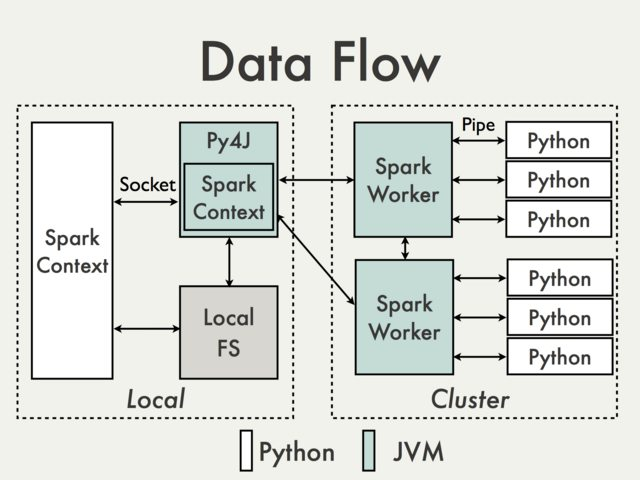
\includegraphics{images/YlI8AqEl.png}
\caption{PySpark Internals}
\end{figure}

\subsection{\texorpdfstring{The \texttt{SparkContext}
class}{The SparkContext class}}\label{the-sparkcontext-class}

\begin{itemize}
\item
  When working with Apache Spark we invoke methods on an object which is
  an instance of the \texttt{pyspark.SparkContext} context.
\item
  Typically, an instance of this object will be created automatically
  for you and assigned to the variable \texttt{sc}.
\item
  The \texttt{parallelize} method in \texttt{SparkContext} can be used
  to turn any ordinary Python collection into an RDD;

  \begin{itemize}
  \tightlist
  \item
    normally we would create an RDD from a large file or an HBase table.
  \end{itemize}
\end{itemize}

    \subsection{First example}\label{first-example}

PySpark isn't on sys.path by default, but that doesn't mean it can't be
used as a regular library. You can address this by either symlinking
pyspark into your site-packages, or adding pyspark to sys.path at
runtime. \href{https://github.com/minrk/findspark}{findspark} does the
latter.

    We have a spark context sc to use with a tiny local spark cluster with 4
nodes (will work just fine on a multicore machine).

    If you use the workstation in room A111 run the code below before:

\begin{Shaded}
\begin{Highlighting}[]
\ImportTok{import}\NormalTok{ findspark}
\ImportTok{import}\NormalTok{ os}
\NormalTok{os.environ[}\StringTok{"JAVA_HOME"}\NormalTok{] }\OperatorTok{=} \StringTok{"/usr/lib/jvm/java-8-openjdk-amd64"}\NormalTok{,}
\NormalTok{os.environ[}\StringTok{"SPARK_HOME"}\NormalTok{] }\OperatorTok{=} \StringTok{"/export/spark-2.3.1-bin-hadoop2.7"}

\NormalTok{findspark.init()}
\end{Highlighting}
\end{Shaded}

    \begin{tcolorbox}[breakable, size=fbox, boxrule=1pt, pad at break*=1mm,colback=cellbackground, colframe=cellborder]
\prompt{In}{incolor}{1}{\boxspacing}
\begin{Verbatim}[commandchars=\\\{\}]
\PY{k+kn}{import} \PY{n+nn}{sys}
\PY{n}{sys}\PY{o}{.}\PY{n}{executable}
\end{Verbatim}
\end{tcolorbox}

            \begin{tcolorbox}[breakable, size=fbox, boxrule=.5pt, pad at break*=1mm, opacityfill=0]
\prompt{Out}{outcolor}{1}{\boxspacing}
\begin{Verbatim}[commandchars=\\\{\}]
'/usr/share/miniconda3/envs/big-data/bin/python'
\end{Verbatim}
\end{tcolorbox}
        
    \begin{tcolorbox}[breakable, size=fbox, boxrule=1pt, pad at break*=1mm,colback=cellbackground, colframe=cellborder]
\prompt{In}{incolor}{2}{\boxspacing}
\begin{Verbatim}[commandchars=\\\{\}]
\PY{k+kn}{import} \PY{n+nn}{sys}\PY{o}{,} \PY{n+nn}{os}
\PY{n}{os}\PY{o}{.}\PY{n}{environ}\PY{p}{[}\PY{l+s+s2}{\PYZdq{}}\PY{l+s+s2}{PYSPARK\PYZus{}PYTHON}\PY{l+s+s2}{\PYZdq{}}\PY{p}{]} \PY{o}{=} \PY{n}{sys}\PY{o}{.}\PY{n}{executable}
\end{Verbatim}
\end{tcolorbox}

    \begin{tcolorbox}[breakable, size=fbox, boxrule=1pt, pad at break*=1mm,colback=cellbackground, colframe=cellborder]
\prompt{In}{incolor}{3}{\boxspacing}
\begin{Verbatim}[commandchars=\\\{\}]
\PY{k+kn}{import} \PY{n+nn}{pyspark}
\end{Verbatim}
\end{tcolorbox}

    \begin{tcolorbox}[breakable, size=fbox, boxrule=1pt, pad at break*=1mm,colback=cellbackground, colframe=cellborder]
\prompt{In}{incolor}{4}{\boxspacing}
\begin{Verbatim}[commandchars=\\\{\}]
\PY{n}{sc} \PY{o}{=} \PY{n}{pyspark}\PY{o}{.}\PY{n}{SparkContext}\PY{p}{(}\PY{n}{master}\PY{o}{=}\PY{l+s+s2}{\PYZdq{}}\PY{l+s+s2}{local[*]}\PY{l+s+s2}{\PYZdq{}}\PY{p}{,} \PY{n}{appName}\PY{o}{=}\PY{l+s+s2}{\PYZdq{}}\PY{l+s+s2}{FirstExample}\PY{l+s+s2}{\PYZdq{}}\PY{p}{)}
\PY{n}{sc}\PY{o}{.}\PY{n}{setLogLevel}\PY{p}{(}\PY{l+s+s2}{\PYZdq{}}\PY{l+s+s2}{ERROR}\PY{l+s+s2}{\PYZdq{}}\PY{p}{)}
\end{Verbatim}
\end{tcolorbox}

    \begin{tcolorbox}[breakable, size=fbox, boxrule=1pt, pad at break*=1mm,colback=cellbackground, colframe=cellborder]
\prompt{In}{incolor}{5}{\boxspacing}
\begin{Verbatim}[commandchars=\\\{\}]
\PY{n+nb}{print}\PY{p}{(}\PY{n}{sc}\PY{p}{)} \PY{c+c1}{\PYZsh{} it is like a Pool Processor executor}
\end{Verbatim}
\end{tcolorbox}

    \begin{Verbatim}[commandchars=\\\{\}]
<SparkContext master=local[*] appName=FirstExample>
    \end{Verbatim}

    \subsection{Create your first RDD}\label{create-your-first-rdd}

    \begin{tcolorbox}[breakable, size=fbox, boxrule=1pt, pad at break*=1mm,colback=cellbackground, colframe=cellborder]
\prompt{In}{incolor}{6}{\boxspacing}
\begin{Verbatim}[commandchars=\\\{\}]
\PY{n}{rdd} \PY{o}{=} \PY{n}{sc}\PY{o}{.}\PY{n}{parallelize}\PY{p}{(}\PY{n+nb}{list}\PY{p}{(}\PY{n+nb}{range}\PY{p}{(}\PY{l+m+mi}{8}\PY{p}{)}\PY{p}{)}\PY{p}{)} \PY{c+c1}{\PYZsh{} create collection}
\end{Verbatim}
\end{tcolorbox}

    \begin{tcolorbox}[breakable, size=fbox, boxrule=1pt, pad at break*=1mm,colback=cellbackground, colframe=cellborder]
\prompt{In}{incolor}{7}{\boxspacing}
\begin{Verbatim}[commandchars=\\\{\}]
\PY{n}{rdd}
\end{Verbatim}
\end{tcolorbox}

            \begin{tcolorbox}[breakable, size=fbox, boxrule=.5pt, pad at break*=1mm, opacityfill=0]
\prompt{Out}{outcolor}{7}{\boxspacing}
\begin{Verbatim}[commandchars=\\\{\}]
ParallelCollectionRDD[0] at readRDDFromFile at PythonRDD.scala:262
\end{Verbatim}
\end{tcolorbox}
        
    \subsubsection{Exercise}\label{exercise}

Create a file \texttt{sample.txt}with lorem package. Read and load it
into a RDD with the \texttt{textFile} spark function.

    \begin{tcolorbox}[breakable, size=fbox, boxrule=1pt, pad at break*=1mm,colback=cellbackground, colframe=cellborder]
\prompt{In}{incolor}{8}{\boxspacing}
\begin{Verbatim}[commandchars=\\\{\}]
\PY{k+kn}{import} \PY{n+nn}{lorem}

\PY{k}{with} \PY{n+nb}{open}\PY{p}{(}\PY{l+s+s2}{\PYZdq{}}\PY{l+s+s2}{sample.txt}\PY{l+s+s2}{\PYZdq{}}\PY{p}{,}\PY{l+s+s2}{\PYZdq{}}\PY{l+s+s2}{w}\PY{l+s+s2}{\PYZdq{}}\PY{p}{)} \PY{k}{as} \PY{n}{f}\PY{p}{:}
    \PY{n}{f}\PY{o}{.}\PY{n}{write}\PY{p}{(}\PY{n}{lorem}\PY{o}{.}\PY{n}{text}\PY{p}{(}\PY{p}{)}\PY{p}{)}
    
\PY{n}{rdd} \PY{o}{=} \PY{n}{sc}\PY{o}{.}\PY{n}{textFile}\PY{p}{(}\PY{l+s+s2}{\PYZdq{}}\PY{l+s+s2}{sample.txt}\PY{l+s+s2}{\PYZdq{}}\PY{p}{)}
\end{Verbatim}
\end{tcolorbox}

    \subsubsection{Collect}\label{collect}

Action / To Driver: Return all items in the RDD to the driver in a
single list

\begin{figure}
\centering
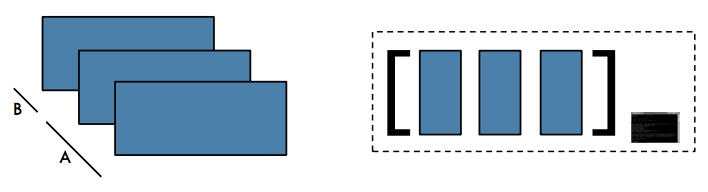
\includegraphics{images/DUO6ygB.png}
\caption{}
\end{figure}

Source: https://i.imgur.com/DUO6ygB.png

\subsubsection{Exercise}\label{exercise}

Collect the text you read before from the \texttt{sample.txt}file.

    \begin{tcolorbox}[breakable, size=fbox, boxrule=1pt, pad at break*=1mm,colback=cellbackground, colframe=cellborder]
\prompt{In}{incolor}{9}{\boxspacing}
\begin{Verbatim}[commandchars=\\\{\}]
\PY{n}{rdd}\PY{o}{.}\PY{n}{collect}\PY{p}{(}\PY{p}{)}
\end{Verbatim}
\end{tcolorbox}

            \begin{tcolorbox}[breakable, size=fbox, boxrule=.5pt, pad at break*=1mm, opacityfill=0]
\prompt{Out}{outcolor}{9}{\boxspacing}
\begin{Verbatim}[commandchars=\\\{\}]
['Dolore quiquia magnam amet eius. Dolorem labore eius etincidunt dolorem magnam
neque est. Magnam tempora quaerat consectetur adipisci. Amet numquam quiquia
dolore aliquam est. Adipisci quaerat ipsum adipisci ipsum sit. Tempora dolor
quisquam est ipsum numquam magnam.',
 '',
 'Etincidunt est est numquam eius sed quiquia non. Dolorem numquam ut quisquam.
Tempora dolore sed eius dolor sed non dolore. Ut eius porro dolorem labore.
Quisquam labore est numquam.',
 '',
 'Ipsum dolor consectetur etincidunt velit. Etincidunt labore labore dolore
quiquia. Magnam eius sed dolore ipsum. Modi modi quaerat dolore. Labore quiquia
sit neque velit. Voluptatem labore quisquam quiquia.',
 '',
 'Labore quisquam porro sit sit ut. Ipsum numquam eius voluptatem amet numquam.
Consectetur adipisci sit non. Dolor velit numquam sit quiquia dolor non. Velit
quaerat consectetur sit dolore. Voluptatem dolor neque dolorem consectetur.']
\end{Verbatim}
\end{tcolorbox}
        
    \subsubsection{Map}\label{map}

Transformation / Narrow: Return a new RDD by applying a function to each
element of this RDD

\begin{figure}
\centering
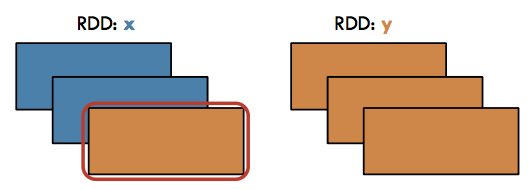
\includegraphics{images/PxNJf0U.png}
\caption{}
\end{figure}

Source: http://i.imgur.com/PxNJf0U.png

    \begin{tcolorbox}[breakable, size=fbox, boxrule=1pt, pad at break*=1mm,colback=cellbackground, colframe=cellborder]
\prompt{In}{incolor}{10}{\boxspacing}
\begin{Verbatim}[commandchars=\\\{\}]
\PY{n}{rdd} \PY{o}{=} \PY{n}{sc}\PY{o}{.}\PY{n}{parallelize}\PY{p}{(}\PY{n+nb}{list}\PY{p}{(}\PY{n+nb}{range}\PY{p}{(}\PY{l+m+mi}{8}\PY{p}{)}\PY{p}{)}\PY{p}{)}
\PY{n}{rdd}\PY{o}{.}\PY{n}{map}\PY{p}{(}\PY{k}{lambda} \PY{n}{x}\PY{p}{:} \PY{n}{x} \PY{o}{*}\PY{o}{*} \PY{l+m+mi}{2}\PY{p}{)}\PY{o}{.}\PY{n}{collect}\PY{p}{(}\PY{p}{)} \PY{c+c1}{\PYZsh{} Square each element}
\end{Verbatim}
\end{tcolorbox}

            \begin{tcolorbox}[breakable, size=fbox, boxrule=.5pt, pad at break*=1mm, opacityfill=0]
\prompt{Out}{outcolor}{10}{\boxspacing}
\begin{Verbatim}[commandchars=\\\{\}]
[0, 1, 4, 9, 16, 25, 36, 49]
\end{Verbatim}
\end{tcolorbox}
        
    \subsubsection{Exercise}\label{exercise}

Replace the lambda function by a function that contains a pause
(sleep(1)) and check if the \texttt{map} operation is parallelized.

    \begin{tcolorbox}[breakable, size=fbox, boxrule=1pt, pad at break*=1mm,colback=cellbackground, colframe=cellborder]
\prompt{In}{incolor}{11}{\boxspacing}
\begin{Verbatim}[commandchars=\\\{\}]
\PY{k+kn}{from} \PY{n+nn}{time} \PY{k+kn}{import} \PY{n}{sleep}
\PY{k}{def} \PY{n+nf}{square}\PY{p}{(}\PY{n}{x}\PY{p}{)}\PY{p}{:}
    \PY{n}{sleep}\PY{p}{(}\PY{l+m+mi}{1}\PY{p}{)}
    \PY{k}{return} \PY{n}{x}\PY{o}{*}\PY{o}{*}\PY{l+m+mi}{2}

\PY{o}{\PYZpc{}}\PY{k}{time} rdd.map(square).collect()
\end{Verbatim}
\end{tcolorbox}

    \begin{Verbatim}[commandchars=\\\{\}]
CPU times: user 2.95 ms, sys: 3.74 ms, total: 6.69 ms
Wall time: 4.06 s
    \end{Verbatim}

            \begin{tcolorbox}[breakable, size=fbox, boxrule=.5pt, pad at break*=1mm, opacityfill=0]
\prompt{Out}{outcolor}{11}{\boxspacing}
\begin{Verbatim}[commandchars=\\\{\}]
[0, 1, 4, 9, 16, 25, 36, 49]
\end{Verbatim}
\end{tcolorbox}
        
    \subsubsection{Filter}\label{filter}

Transformation / Narrow: Return a new RDD containing only the elements
that satisfy a predicate

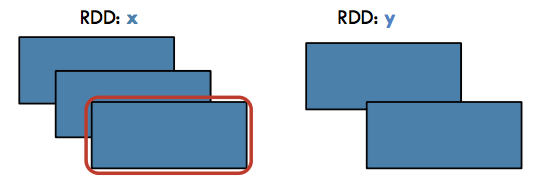
\includegraphics{images/GFyji4U.png} Source:
http://i.imgur.com/GFyji4U.png

    \begin{tcolorbox}[breakable, size=fbox, boxrule=1pt, pad at break*=1mm,colback=cellbackground, colframe=cellborder]
\prompt{In}{incolor}{12}{\boxspacing}
\begin{Verbatim}[commandchars=\\\{\}]
\PY{c+c1}{\PYZsh{} Select only the even elements}
\PY{n}{rdd}\PY{o}{.}\PY{n}{filter}\PY{p}{(}\PY{k}{lambda} \PY{n}{x}\PY{p}{:} \PY{n}{x} \PY{o}{\PYZpc{}} \PY{l+m+mi}{2} \PY{o}{==} \PY{l+m+mi}{0}\PY{p}{)}\PY{o}{.}\PY{n}{collect}\PY{p}{(}\PY{p}{)}
\end{Verbatim}
\end{tcolorbox}

            \begin{tcolorbox}[breakable, size=fbox, boxrule=.5pt, pad at break*=1mm, opacityfill=0]
\prompt{Out}{outcolor}{12}{\boxspacing}
\begin{Verbatim}[commandchars=\\\{\}]
[0, 2, 4, 6]
\end{Verbatim}
\end{tcolorbox}
        
    \subsubsection{FlatMap}\label{flatmap}

Transformation / Narrow: Return a new RDD by first applying a function
to all elements of this RDD, and then flattening the results

\begin{figure}
\centering
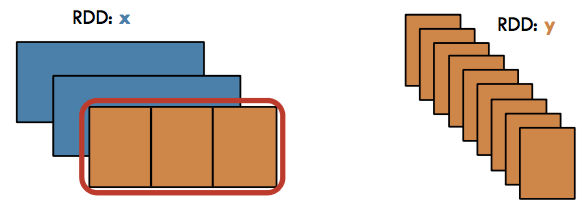
\includegraphics{images/TsSUex8.png}
\caption{}
\end{figure}

    \begin{tcolorbox}[breakable, size=fbox, boxrule=1pt, pad at break*=1mm,colback=cellbackground, colframe=cellborder]
\prompt{In}{incolor}{13}{\boxspacing}
\begin{Verbatim}[commandchars=\\\{\}]
\PY{n}{rdd} \PY{o}{=} \PY{n}{sc}\PY{o}{.}\PY{n}{parallelize}\PY{p}{(}\PY{p}{[}\PY{l+m+mi}{1}\PY{p}{,}\PY{l+m+mi}{2}\PY{p}{,}\PY{l+m+mi}{3}\PY{p}{]}\PY{p}{)}
\PY{n}{rdd}\PY{o}{.}\PY{n}{flatMap}\PY{p}{(}\PY{k}{lambda} \PY{n}{x}\PY{p}{:} \PY{p}{(}\PY{n}{x}\PY{p}{,} \PY{n}{x}\PY{o}{*}\PY{l+m+mi}{100}\PY{p}{,} \PY{l+m+mi}{42}\PY{p}{)}\PY{p}{)}\PY{o}{.}\PY{n}{collect}\PY{p}{(}\PY{p}{)}
\end{Verbatim}
\end{tcolorbox}

            \begin{tcolorbox}[breakable, size=fbox, boxrule=.5pt, pad at break*=1mm, opacityfill=0]
\prompt{Out}{outcolor}{13}{\boxspacing}
\begin{Verbatim}[commandchars=\\\{\}]
[1, 100, 42, 2, 200, 42, 3, 300, 42]
\end{Verbatim}
\end{tcolorbox}
        
    \subsubsection{Exercise}\label{exercise}

Use FlatMap to clean the text from \texttt{sample.txt}file. Lower,
remove dots and split into words.

\subsubsection{GroupBy}\label{groupby}

Transformation / Wide: Group the data in the original RDD. Create pairs
where the key is the output of a user function, and the value is all
items for which the function yields this key.

\begin{figure}
\centering
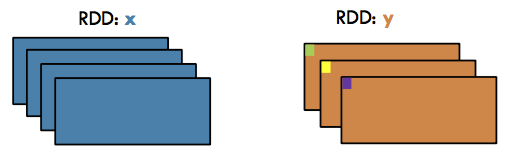
\includegraphics{images/gdj0Ey8.png}
\caption{}
\end{figure}

    \begin{tcolorbox}[breakable, size=fbox, boxrule=1pt, pad at break*=1mm,colback=cellbackground, colframe=cellborder]
\prompt{In}{incolor}{14}{\boxspacing}
\begin{Verbatim}[commandchars=\\\{\}]
\PY{n}{rdd} \PY{o}{=} \PY{n}{sc}\PY{o}{.}\PY{n}{parallelize}\PY{p}{(}\PY{p}{[}\PY{l+s+s1}{\PYZsq{}}\PY{l+s+s1}{John}\PY{l+s+s1}{\PYZsq{}}\PY{p}{,} \PY{l+s+s1}{\PYZsq{}}\PY{l+s+s1}{Fred}\PY{l+s+s1}{\PYZsq{}}\PY{p}{,} \PY{l+s+s1}{\PYZsq{}}\PY{l+s+s1}{Anna}\PY{l+s+s1}{\PYZsq{}}\PY{p}{,} \PY{l+s+s1}{\PYZsq{}}\PY{l+s+s1}{James}\PY{l+s+s1}{\PYZsq{}}\PY{p}{]}\PY{p}{)}
\PY{n}{rdd} \PY{o}{=} \PY{n}{rdd}\PY{o}{.}\PY{n}{groupBy}\PY{p}{(}\PY{k}{lambda} \PY{n}{w}\PY{p}{:} \PY{n}{w}\PY{p}{[}\PY{l+m+mi}{0}\PY{p}{]}\PY{p}{)}
\PY{p}{[}\PY{p}{(}\PY{n}{k}\PY{p}{,} \PY{n+nb}{list}\PY{p}{(}\PY{n}{v}\PY{p}{)}\PY{p}{)} \PY{k}{for} \PY{p}{(}\PY{n}{k}\PY{p}{,} \PY{n}{v}\PY{p}{)} \PY{o+ow}{in} \PY{n}{rdd}\PY{o}{.}\PY{n}{collect}\PY{p}{(}\PY{p}{)}\PY{p}{]}
\end{Verbatim}
\end{tcolorbox}

            \begin{tcolorbox}[breakable, size=fbox, boxrule=.5pt, pad at break*=1mm, opacityfill=0]
\prompt{Out}{outcolor}{14}{\boxspacing}
\begin{Verbatim}[commandchars=\\\{\}]
[('J', ['John', 'James']), ('F', ['Fred']), ('A', ['Anna'])]
\end{Verbatim}
\end{tcolorbox}
        
    \subsubsection{GroupByKey}\label{groupbykey}

Transformation / Wide: Group the values for each key in the original
RDD. Create a new pair where the original key corresponds to this
collected group of values.

\begin{figure}
\centering
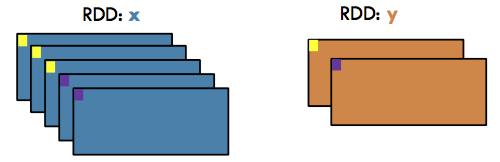
\includegraphics{images/TlWRGr2.png}
\caption{}
\end{figure}

    \begin{tcolorbox}[breakable, size=fbox, boxrule=1pt, pad at break*=1mm,colback=cellbackground, colframe=cellborder]
\prompt{In}{incolor}{15}{\boxspacing}
\begin{Verbatim}[commandchars=\\\{\}]
\PY{n}{rdd} \PY{o}{=} \PY{n}{sc}\PY{o}{.}\PY{n}{parallelize}\PY{p}{(}\PY{p}{[}\PY{p}{(}\PY{l+s+s1}{\PYZsq{}}\PY{l+s+s1}{B}\PY{l+s+s1}{\PYZsq{}}\PY{p}{,}\PY{l+m+mi}{5}\PY{p}{)}\PY{p}{,}\PY{p}{(}\PY{l+s+s1}{\PYZsq{}}\PY{l+s+s1}{B}\PY{l+s+s1}{\PYZsq{}}\PY{p}{,}\PY{l+m+mi}{4}\PY{p}{)}\PY{p}{,}\PY{p}{(}\PY{l+s+s1}{\PYZsq{}}\PY{l+s+s1}{A}\PY{l+s+s1}{\PYZsq{}}\PY{p}{,}\PY{l+m+mi}{3}\PY{p}{)}\PY{p}{,}\PY{p}{(}\PY{l+s+s1}{\PYZsq{}}\PY{l+s+s1}{A}\PY{l+s+s1}{\PYZsq{}}\PY{p}{,}\PY{l+m+mi}{2}\PY{p}{)}\PY{p}{,}\PY{p}{(}\PY{l+s+s1}{\PYZsq{}}\PY{l+s+s1}{A}\PY{l+s+s1}{\PYZsq{}}\PY{p}{,}\PY{l+m+mi}{1}\PY{p}{)}\PY{p}{]}\PY{p}{)}
\PY{n}{rdd} \PY{o}{=} \PY{n}{rdd}\PY{o}{.}\PY{n}{groupByKey}\PY{p}{(}\PY{p}{)}
\PY{p}{[}\PY{p}{(}\PY{n}{j}\PY{p}{[}\PY{l+m+mi}{0}\PY{p}{]}\PY{p}{,} \PY{n+nb}{list}\PY{p}{(}\PY{n}{j}\PY{p}{[}\PY{l+m+mi}{1}\PY{p}{]}\PY{p}{)}\PY{p}{)} \PY{k}{for} \PY{n}{j} \PY{o+ow}{in} \PY{n}{rdd}\PY{o}{.}\PY{n}{collect}\PY{p}{(}\PY{p}{)}\PY{p}{]}
\end{Verbatim}
\end{tcolorbox}

            \begin{tcolorbox}[breakable, size=fbox, boxrule=.5pt, pad at break*=1mm, opacityfill=0]
\prompt{Out}{outcolor}{15}{\boxspacing}
\begin{Verbatim}[commandchars=\\\{\}]
[('B', [5, 4]), ('A', [3, 2, 1])]
\end{Verbatim}
\end{tcolorbox}
        
    \subsubsection{Join}\label{join}

Transformation / Wide: Return a new RDD containing all pairs of elements
having the same key in the original RDDs

\begin{figure}
\centering
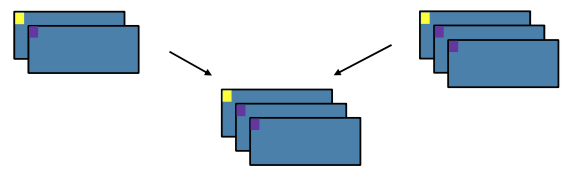
\includegraphics{images/YXL42Nl.png}
\caption{}
\end{figure}

    \begin{tcolorbox}[breakable, size=fbox, boxrule=1pt, pad at break*=1mm,colback=cellbackground, colframe=cellborder]
\prompt{In}{incolor}{16}{\boxspacing}
\begin{Verbatim}[commandchars=\\\{\}]
\PY{n}{x} \PY{o}{=} \PY{n}{sc}\PY{o}{.}\PY{n}{parallelize}\PY{p}{(}\PY{p}{[}\PY{p}{(}\PY{l+s+s2}{\PYZdq{}}\PY{l+s+s2}{a}\PY{l+s+s2}{\PYZdq{}}\PY{p}{,} \PY{l+m+mi}{1}\PY{p}{)}\PY{p}{,} \PY{p}{(}\PY{l+s+s2}{\PYZdq{}}\PY{l+s+s2}{b}\PY{l+s+s2}{\PYZdq{}}\PY{p}{,} \PY{l+m+mi}{2}\PY{p}{)}\PY{p}{]}\PY{p}{)}
\PY{n}{y} \PY{o}{=} \PY{n}{sc}\PY{o}{.}\PY{n}{parallelize}\PY{p}{(}\PY{p}{[}\PY{p}{(}\PY{l+s+s2}{\PYZdq{}}\PY{l+s+s2}{a}\PY{l+s+s2}{\PYZdq{}}\PY{p}{,} \PY{l+m+mi}{3}\PY{p}{)}\PY{p}{,} \PY{p}{(}\PY{l+s+s2}{\PYZdq{}}\PY{l+s+s2}{a}\PY{l+s+s2}{\PYZdq{}}\PY{p}{,} \PY{l+m+mi}{4}\PY{p}{)}\PY{p}{,} \PY{p}{(}\PY{l+s+s2}{\PYZdq{}}\PY{l+s+s2}{b}\PY{l+s+s2}{\PYZdq{}}\PY{p}{,} \PY{l+m+mi}{5}\PY{p}{)}\PY{p}{]}\PY{p}{)}
\PY{n}{x}\PY{o}{.}\PY{n}{join}\PY{p}{(}\PY{n}{y}\PY{p}{)}\PY{o}{.}\PY{n}{collect}\PY{p}{(}\PY{p}{)}
\end{Verbatim}
\end{tcolorbox}

            \begin{tcolorbox}[breakable, size=fbox, boxrule=.5pt, pad at break*=1mm, opacityfill=0]
\prompt{Out}{outcolor}{16}{\boxspacing}
\begin{Verbatim}[commandchars=\\\{\}]
[('b', (2, 5)), ('a', (1, 3)), ('a', (1, 4))]
\end{Verbatim}
\end{tcolorbox}
        
    \subsubsection{Distinct}\label{distinct}

Transformation / Wide: Return a new RDD containing distinct items from
the original RDD (omitting all duplicates)

\begin{figure}
\centering
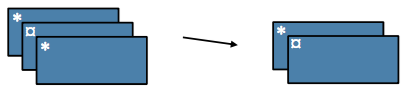
\includegraphics{images/Vqgy2a4.png}
\caption{}
\end{figure}

    \begin{tcolorbox}[breakable, size=fbox, boxrule=1pt, pad at break*=1mm,colback=cellbackground, colframe=cellborder]
\prompt{In}{incolor}{17}{\boxspacing}
\begin{Verbatim}[commandchars=\\\{\}]
\PY{n}{rdd} \PY{o}{=} \PY{n}{sc}\PY{o}{.}\PY{n}{parallelize}\PY{p}{(}\PY{p}{[}\PY{l+m+mi}{1}\PY{p}{,}\PY{l+m+mi}{2}\PY{p}{,}\PY{l+m+mi}{3}\PY{p}{,}\PY{l+m+mi}{3}\PY{p}{,}\PY{l+m+mi}{4}\PY{p}{]}\PY{p}{)}
\PY{n}{rdd}\PY{o}{.}\PY{n}{distinct}\PY{p}{(}\PY{p}{)}\PY{o}{.}\PY{n}{collect}\PY{p}{(}\PY{p}{)}
\end{Verbatim}
\end{tcolorbox}

            \begin{tcolorbox}[breakable, size=fbox, boxrule=.5pt, pad at break*=1mm, opacityfill=0]
\prompt{Out}{outcolor}{17}{\boxspacing}
\begin{Verbatim}[commandchars=\\\{\}]
[2, 4, 1, 3]
\end{Verbatim}
\end{tcolorbox}
        
    \subsubsection{KeyBy}\label{keyby}

Transformation / Narrow: Create a Pair RDD, forming one pair for each
item in the original RDD. The pair's key is calculated from the value
via a user-supplied function.

\begin{figure}
\centering
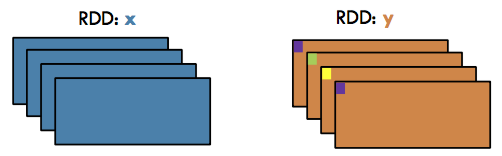
\includegraphics{images/nqYhDW5.png}
\caption{}
\end{figure}

    \begin{tcolorbox}[breakable, size=fbox, boxrule=1pt, pad at break*=1mm,colback=cellbackground, colframe=cellborder]
\prompt{In}{incolor}{18}{\boxspacing}
\begin{Verbatim}[commandchars=\\\{\}]
\PY{n}{rdd} \PY{o}{=} \PY{n}{sc}\PY{o}{.}\PY{n}{parallelize}\PY{p}{(}\PY{p}{[}\PY{l+s+s1}{\PYZsq{}}\PY{l+s+s1}{John}\PY{l+s+s1}{\PYZsq{}}\PY{p}{,} \PY{l+s+s1}{\PYZsq{}}\PY{l+s+s1}{Fred}\PY{l+s+s1}{\PYZsq{}}\PY{p}{,} \PY{l+s+s1}{\PYZsq{}}\PY{l+s+s1}{Anna}\PY{l+s+s1}{\PYZsq{}}\PY{p}{,} \PY{l+s+s1}{\PYZsq{}}\PY{l+s+s1}{James}\PY{l+s+s1}{\PYZsq{}}\PY{p}{]}\PY{p}{)}
\PY{n}{rdd}\PY{o}{.}\PY{n}{keyBy}\PY{p}{(}\PY{k}{lambda} \PY{n}{w}\PY{p}{:} \PY{n}{w}\PY{p}{[}\PY{l+m+mi}{0}\PY{p}{]}\PY{p}{)}\PY{o}{.}\PY{n}{collect}\PY{p}{(}\PY{p}{)}
\end{Verbatim}
\end{tcolorbox}

            \begin{tcolorbox}[breakable, size=fbox, boxrule=.5pt, pad at break*=1mm, opacityfill=0]
\prompt{Out}{outcolor}{18}{\boxspacing}
\begin{Verbatim}[commandchars=\\\{\}]
[('J', 'John'), ('F', 'Fred'), ('A', 'Anna'), ('J', 'James')]
\end{Verbatim}
\end{tcolorbox}
        
    \subsection{Actions}\label{actions}

\subsubsection{Map-Reduce operation}\label{map-reduce-operation}

Action / To Driver: Aggregate all the elements of the RDD by applying a
user function pairwise to elements and partial results, and return a
result to the driver

\begin{figure}
\centering
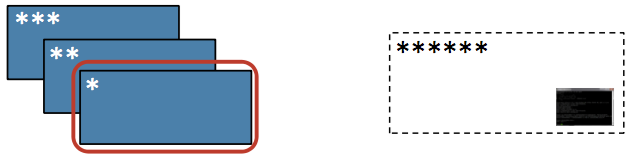
\includegraphics{images/R72uzwX.png}
\caption{}
\end{figure}

    \begin{tcolorbox}[breakable, size=fbox, boxrule=1pt, pad at break*=1mm,colback=cellbackground, colframe=cellborder]
\prompt{In}{incolor}{19}{\boxspacing}
\begin{Verbatim}[commandchars=\\\{\}]
\PY{k+kn}{from} \PY{n+nn}{operator} \PY{k+kn}{import} \PY{n}{add}
\PY{n}{rdd} \PY{o}{=} \PY{n}{sc}\PY{o}{.}\PY{n}{parallelize}\PY{p}{(}\PY{n+nb}{list}\PY{p}{(}\PY{n+nb}{range}\PY{p}{(}\PY{l+m+mi}{8}\PY{p}{)}\PY{p}{)}\PY{p}{)}
\PY{n}{rdd}\PY{o}{.}\PY{n}{map}\PY{p}{(}\PY{k}{lambda} \PY{n}{x}\PY{p}{:} \PY{n}{x} \PY{o}{*}\PY{o}{*} \PY{l+m+mi}{2}\PY{p}{)}\PY{o}{.}\PY{n}{reduce}\PY{p}{(}\PY{n}{add}\PY{p}{)} \PY{c+c1}{\PYZsh{} reduce is an action!}
\end{Verbatim}
\end{tcolorbox}

            \begin{tcolorbox}[breakable, size=fbox, boxrule=.5pt, pad at break*=1mm, opacityfill=0]
\prompt{Out}{outcolor}{19}{\boxspacing}
\begin{Verbatim}[commandchars=\\\{\}]
140
\end{Verbatim}
\end{tcolorbox}
        
    \subsubsection{Max, Min, Sum, Mean, Variance,
Stdev}\label{max-min-sum-mean-variance-stdev}

Action / To Driver: Compute the respective function (maximum value,
minimum value, sum, mean, variance, or standard deviation) from a
numeric RDD

\begin{figure}
\centering
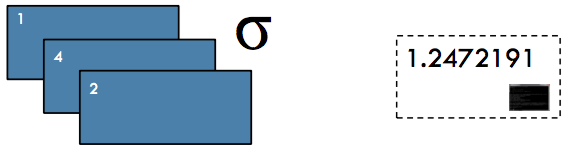
\includegraphics{images/HUCtib1.png}
\caption{}
\end{figure}

    \subsubsection{CountByKey}\label{countbykey}

Action / To Driver: Return a map of keys and counts of their occurrences
in the RDD

\begin{figure}
\centering
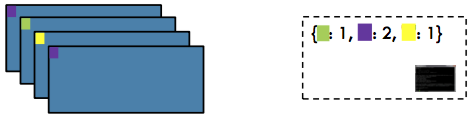
\includegraphics{images/jvQTGv6.png}
\caption{}
\end{figure}

    \begin{tcolorbox}[breakable, size=fbox, boxrule=1pt, pad at break*=1mm,colback=cellbackground, colframe=cellborder]
\prompt{In}{incolor}{20}{\boxspacing}
\begin{Verbatim}[commandchars=\\\{\}]
\PY{n}{rdd} \PY{o}{=} \PY{n}{sc}\PY{o}{.}\PY{n}{parallelize}\PY{p}{(}\PY{p}{[}\PY{p}{(}\PY{l+s+s1}{\PYZsq{}}\PY{l+s+s1}{J}\PY{l+s+s1}{\PYZsq{}}\PY{p}{,} \PY{l+s+s1}{\PYZsq{}}\PY{l+s+s1}{James}\PY{l+s+s1}{\PYZsq{}}\PY{p}{)}\PY{p}{,} \PY{p}{(}\PY{l+s+s1}{\PYZsq{}}\PY{l+s+s1}{F}\PY{l+s+s1}{\PYZsq{}}\PY{p}{,}\PY{l+s+s1}{\PYZsq{}}\PY{l+s+s1}{Fred}\PY{l+s+s1}{\PYZsq{}}\PY{p}{)}\PY{p}{,} 
                    \PY{p}{(}\PY{l+s+s1}{\PYZsq{}}\PY{l+s+s1}{A}\PY{l+s+s1}{\PYZsq{}}\PY{p}{,}\PY{l+s+s1}{\PYZsq{}}\PY{l+s+s1}{Anna}\PY{l+s+s1}{\PYZsq{}}\PY{p}{)}\PY{p}{,} \PY{p}{(}\PY{l+s+s1}{\PYZsq{}}\PY{l+s+s1}{J}\PY{l+s+s1}{\PYZsq{}}\PY{p}{,}\PY{l+s+s1}{\PYZsq{}}\PY{l+s+s1}{John}\PY{l+s+s1}{\PYZsq{}}\PY{p}{)}\PY{p}{]}\PY{p}{)}

\PY{n}{rdd}\PY{o}{.}\PY{n}{countByKey}\PY{p}{(}\PY{p}{)}
\end{Verbatim}
\end{tcolorbox}

            \begin{tcolorbox}[breakable, size=fbox, boxrule=.5pt, pad at break*=1mm, opacityfill=0]
\prompt{Out}{outcolor}{20}{\boxspacing}
\begin{Verbatim}[commandchars=\\\{\}]
defaultdict(int, \{'J': 2, 'F': 1, 'A': 1\})
\end{Verbatim}
\end{tcolorbox}
        
    \begin{tcolorbox}[breakable, size=fbox, boxrule=1pt, pad at break*=1mm,colback=cellbackground, colframe=cellborder]
\prompt{In}{incolor}{21}{\boxspacing}
\begin{Verbatim}[commandchars=\\\{\}]
\PY{c+c1}{\PYZsh{} Stop the local spark cluster}
\PY{n}{sc}\PY{o}{.}\PY{n}{stop}\PY{p}{(}\PY{p}{)}
\end{Verbatim}
\end{tcolorbox}

    \subsubsection{Exercise 10.1 Word-count in Apache
Spark}\label{exercise-10.1-word-count-in-apache-spark}

\begin{itemize}
\tightlist
\item
  Write the sample text file
\end{itemize}

    \begin{tcolorbox}[breakable, size=fbox, boxrule=1pt, pad at break*=1mm,colback=cellbackground, colframe=cellborder]
\prompt{In}{incolor}{22}{\boxspacing}
\begin{Verbatim}[commandchars=\\\{\}]
\PY{k+kn}{from} \PY{n+nn}{lorem} \PY{k+kn}{import} \PY{n}{text}
\PY{k}{with} \PY{n+nb}{open}\PY{p}{(}\PY{l+s+s1}{\PYZsq{}}\PY{l+s+s1}{sample.txt}\PY{l+s+s1}{\PYZsq{}}\PY{p}{,}\PY{l+s+s1}{\PYZsq{}}\PY{l+s+s1}{w}\PY{l+s+s1}{\PYZsq{}}\PY{p}{)} \PY{k}{as} \PY{n}{f}\PY{p}{:}
    \PY{n}{f}\PY{o}{.}\PY{n}{write}\PY{p}{(}\PY{n}{text}\PY{p}{(}\PY{p}{)}\PY{p}{)}
\end{Verbatim}
\end{tcolorbox}

    \begin{itemize}
\tightlist
\item
  Create the rdd with \texttt{SparkContext.textFile\ method}
\item
  lower, remove dots and split using \texttt{rdd.flatMap}
\item
  use \texttt{rdd.map} to create the list of key/value pair (word, 1)
\item
  \texttt{rdd.reduceByKey} to get all occurences
\item
  \texttt{rdd.takeOrdered}to get sorted frequencies of words
\end{itemize}

All documentation is available
\href{https://spark.apache.org/docs/2.1.0/api/python/pyspark.html?highlight=textfile\#pyspark.SparkContext}{here}
for textFile and
\href{https://spark.apache.org/docs/2.1.0/api/python/pyspark.html?highlight=textfile\#pyspark.RDD}{here}
for RDD.

For a global overview see the Transformations section of the
\href{https://spark.apache.org/docs/latest/rdd-programming-guide.html}{programming
guide}

    \begin{tcolorbox}[breakable, size=fbox, boxrule=1pt, pad at break*=1mm,colback=cellbackground, colframe=cellborder]
\prompt{In}{incolor}{23}{\boxspacing}
\begin{Verbatim}[commandchars=\\\{\}]
\PY{k+kn}{import} \PY{n+nn}{pyspark}

\PY{n}{sc} \PY{o}{=} \PY{n}{pyspark}\PY{o}{.}\PY{n}{SparkContext}\PY{p}{(}\PY{n}{master}\PY{o}{=}\PY{l+s+s2}{\PYZdq{}}\PY{l+s+s2}{local[*]}\PY{l+s+s2}{\PYZdq{}}\PY{p}{,} \PY{n}{appName}\PY{o}{=}\PY{l+s+s2}{\PYZdq{}}\PY{l+s+s2}{wordcount}\PY{l+s+s2}{\PYZdq{}}\PY{p}{)}
\PY{n}{sc}\PY{o}{.}\PY{n}{setLogLevel}\PY{p}{(}\PY{l+s+s2}{\PYZdq{}}\PY{l+s+s2}{ERROR}\PY{l+s+s2}{\PYZdq{}}\PY{p}{)}
\end{Verbatim}
\end{tcolorbox}

    \begin{tcolorbox}[breakable, size=fbox, boxrule=1pt, pad at break*=1mm,colback=cellbackground, colframe=cellborder]
\prompt{In}{incolor}{24}{\boxspacing}
\begin{Verbatim}[commandchars=\\\{\}]
\PY{n}{rdd} \PY{o}{=} \PY{n}{sc}\PY{o}{.}\PY{n}{textFile}\PY{p}{(}\PY{l+s+s2}{\PYZdq{}}\PY{l+s+s2}{sample.txt}\PY{l+s+s2}{\PYZdq{}}\PY{p}{)}
\end{Verbatim}
\end{tcolorbox}

    \begin{tcolorbox}[breakable, size=fbox, boxrule=1pt, pad at break*=1mm,colback=cellbackground, colframe=cellborder]
\prompt{In}{incolor}{25}{\boxspacing}
\begin{Verbatim}[commandchars=\\\{\}]
\PY{p}{(}\PY{n}{rdd}\PY{o}{.}\PY{n}{flatMap}\PY{p}{(}\PY{k}{lambda} \PY{n}{line}\PY{p}{:} \PY{n}{line}\PY{o}{.}\PY{n}{lower}\PY{p}{(}\PY{p}{)}\PY{o}{.}\PY{n}{replace}\PY{p}{(}\PY{l+s+s2}{\PYZdq{}}\PY{l+s+s2}{.}\PY{l+s+s2}{\PYZdq{}}\PY{p}{,}\PY{l+s+s2}{\PYZdq{}}\PY{l+s+s2}{ }\PY{l+s+s2}{\PYZdq{}}\PY{p}{)}\PY{o}{.}\PY{n}{split}\PY{p}{(}\PY{p}{)}\PY{p}{)}
   \PY{o}{.}\PY{n}{map}\PY{p}{(}\PY{k}{lambda} \PY{n}{w} \PY{p}{:} \PY{p}{(}\PY{n}{w}\PY{p}{,}\PY{l+m+mi}{1}\PY{p}{)}\PY{p}{)}
   \PY{o}{.}\PY{n}{reduceByKey}\PY{p}{(}\PY{k}{lambda} \PY{n}{w}\PY{p}{,} \PY{n}{c}\PY{p}{:} \PY{n}{w} \PY{o}{+} \PY{n}{c}\PY{p}{)}
   \PY{o}{.}\PY{n}{sortBy}\PY{p}{(} \PY{k}{lambda} \PY{n}{w} \PY{p}{:} \PY{o}{\PYZhy{}}\PY{n}{w}\PY{p}{[}\PY{l+m+mi}{1}\PY{p}{]}\PY{p}{)}\PY{o}{.}\PY{n}{collect}\PY{p}{(}\PY{p}{)}\PY{p}{)}
\end{Verbatim}
\end{tcolorbox}

            \begin{tcolorbox}[breakable, size=fbox, boxrule=.5pt, pad at break*=1mm, opacityfill=0]
\prompt{Out}{outcolor}{25}{\boxspacing}
\begin{Verbatim}[commandchars=\\\{\}]
[('porro', 14),
 ('sed', 14),
 ('eius', 13),
 ('est', 12),
 ('consectetur', 11),
 ('velit', 11),
 ('numquam', 11),
 ('modi', 10),
 ('neque', 10),
 ('etincidunt', 10),
 ('aliquam', 10),
 ('tempora', 9),
 ('magnam', 9),
 ('labore', 9),
 ('dolor', 9),
 ('adipisci', 8),
 ('ut', 8),
 ('quaerat', 7),
 ('dolore', 6),
 ('quisquam', 6),
 ('non', 6),
 ('ipsum', 5),
 ('dolorem', 5),
 ('sit', 5),
 ('amet', 4),
 ('quiquia', 3),
 ('voluptatem', 3)]
\end{Verbatim}
\end{tcolorbox}
        
    \begin{tcolorbox}[breakable, size=fbox, boxrule=1pt, pad at break*=1mm,colback=cellbackground, colframe=cellborder]
\prompt{In}{incolor}{26}{\boxspacing}
\begin{Verbatim}[commandchars=\\\{\}]
\PY{n}{sc}\PY{o}{.}\PY{n}{stop}\PY{p}{(}\PY{p}{)}
\end{Verbatim}
\end{tcolorbox}

    \subsection{SparkSession}\label{sparksession}

Since SPARK 2.0.0, SparkSession provides a single point of entry to
interact with Spark functionality and allows programming Spark with
DataFrame and Dataset APIs.

\subsubsection{\texorpdfstring{\(\pi\) computation
example}{\textbackslash{}pi computation example}}\label{pi-computation-example}

\begin{itemize}
\tightlist
\item
  We can estimate an approximate value for \(\pi\) using the following
  Monte-Carlo method:
\end{itemize}

\begin{enumerate}
\def\labelenumi{\arabic{enumi}.}
\tightlist
\item
  Inscribe a circle in a square
\item
  Randomly generate points in the square
\item
  Determine the number of points in the square that are also in the
  circle
\item
  Let \(r\) be the number of points in the circle divided by the number
  of points in the square, then \(\pi \approx 4 r\).
\end{enumerate}

\begin{itemize}
\tightlist
\item
  Note that the more points generated, the better the approximation
\end{itemize}

See
\href{https://computing.llnl.gov/tutorials/parallel_comp/\#ExamplesPI}{this
tutorial}.

    \begin{tcolorbox}[breakable, size=fbox, boxrule=1pt, pad at break*=1mm,colback=cellbackground, colframe=cellborder]
\prompt{In}{incolor}{27}{\boxspacing}
\begin{Verbatim}[commandchars=\\\{\}]
\PY{k+kn}{import} \PY{n+nn}{sys}
\PY{k+kn}{from} \PY{n+nn}{random} \PY{k+kn}{import} \PY{n}{random}
\PY{k+kn}{from} \PY{n+nn}{operator} \PY{k+kn}{import} \PY{n}{add}

\PY{k+kn}{from} \PY{n+nn}{pyspark}\PY{n+nn}{.}\PY{n+nn}{sql} \PY{k+kn}{import} \PY{n}{SparkSession}

\PY{n}{spark} \PY{o}{=} \PY{p}{(}\PY{n}{SparkSession}\PY{o}{.}\PY{n}{builder}\PY{o}{.}\PY{n}{master}\PY{p}{(}\PY{l+s+s2}{\PYZdq{}}\PY{l+s+s2}{local[*]}\PY{l+s+s2}{\PYZdq{}}\PY{p}{)}
         \PY{o}{.}\PY{n}{appName}\PY{p}{(}\PY{l+s+s2}{\PYZdq{}}\PY{l+s+s2}{PythonPi}\PY{l+s+s2}{\PYZdq{}}\PY{p}{)}
         \PY{o}{.}\PY{n}{getOrCreate}\PY{p}{(}\PY{p}{)}\PY{p}{)}

\PY{n}{partitions} \PY{o}{=} \PY{l+m+mi}{8}
\PY{n}{n} \PY{o}{=} \PY{l+m+mi}{100000} \PY{o}{*} \PY{n}{partitions}

\PY{k}{def} \PY{n+nf}{f}\PY{p}{(}\PY{n}{\PYZus{}}\PY{p}{)}\PY{p}{:}
    \PY{n}{x} \PY{o}{=} \PY{n}{random}\PY{p}{(}\PY{p}{)} \PY{o}{*} \PY{l+m+mi}{2} \PY{o}{\PYZhy{}} \PY{l+m+mi}{1}
    \PY{n}{y} \PY{o}{=} \PY{n}{random}\PY{p}{(}\PY{p}{)} \PY{o}{*} \PY{l+m+mi}{2} \PY{o}{\PYZhy{}} \PY{l+m+mi}{1}
    \PY{k}{return} \PY{l+m+mi}{1} \PY{k}{if} \PY{n}{x} \PY{o}{*}\PY{o}{*} \PY{l+m+mi}{2} \PY{o}{+} \PY{n}{y} \PY{o}{*}\PY{o}{*} \PY{l+m+mi}{2} \PY{o}{\PYZlt{}}\PY{o}{=} \PY{l+m+mi}{1} \PY{k}{else} \PY{l+m+mi}{0}

\PY{n}{count} \PY{o}{=} \PY{n}{spark}\PY{o}{.}\PY{n}{sparkContext}\PY{o}{.}\PY{n}{parallelize}\PY{p}{(}\PY{n+nb}{range}\PY{p}{(}\PY{l+m+mi}{1}\PY{p}{,} \PY{n}{n}\PY{o}{+}\PY{l+m+mi}{1}\PY{p}{)}\PY{p}{,} \PY{n}{partitions}\PY{p}{)}\PY{o}{.}\PY{n}{map}\PY{p}{(}\PY{n}{f}\PY{p}{)}\PY{o}{.}\PY{n}{reduce}\PY{p}{(}\PY{n}{add}\PY{p}{)}
\PY{n+nb}{print}\PY{p}{(}\PY{l+s+s2}{\PYZdq{}}\PY{l+s+s2}{Pi is roughly }\PY{l+s+si}{\PYZpc{}f}\PY{l+s+s2}{\PYZdq{}} \PY{o}{\PYZpc{}} \PY{p}{(}\PY{l+m+mf}{4.0} \PY{o}{*} \PY{n}{count} \PY{o}{/} \PY{n}{n}\PY{p}{)}\PY{p}{)}

\PY{n}{spark}\PY{o}{.}\PY{n}{stop}\PY{p}{(}\PY{p}{)}
\end{Verbatim}
\end{tcolorbox}

    \begin{Verbatim}[commandchars=\\\{\}]
Pi is roughly 3.143145
    \end{Verbatim}

    \subsubsection{Exercise 9.2}\label{exercise-9.2}

Using the same method than the PI computation example, compute the
integral \[
I = \int_0^1 \exp(-x^2) dx
\] You can check your result with numpy

    \begin{tcolorbox}[breakable, size=fbox, boxrule=1pt, pad at break*=1mm,colback=cellbackground, colframe=cellborder]
\prompt{In}{incolor}{28}{\boxspacing}
\begin{Verbatim}[commandchars=\\\{\}]
\PY{c+c1}{\PYZsh{} numpy evaluates solution using numeric computation. }
\PY{c+c1}{\PYZsh{} It uses discrete values of the function}
\PY{k+kn}{import} \PY{n+nn}{numpy} \PY{k}{as} \PY{n+nn}{np}
\PY{n}{x} \PY{o}{=} \PY{n}{np}\PY{o}{.}\PY{n}{linspace}\PY{p}{(}\PY{l+m+mi}{0}\PY{p}{,}\PY{l+m+mi}{1}\PY{p}{,}\PY{l+m+mi}{1000}\PY{p}{)}
\PY{n}{np}\PY{o}{.}\PY{n}{trapz}\PY{p}{(}\PY{n}{np}\PY{o}{.}\PY{n}{exp}\PY{p}{(}\PY{o}{\PYZhy{}}\PY{n}{x}\PY{o}{*}\PY{n}{x}\PY{p}{)}\PY{p}{,}\PY{n}{x}\PY{p}{)}
\end{Verbatim}
\end{tcolorbox}

            \begin{tcolorbox}[breakable, size=fbox, boxrule=.5pt, pad at break*=1mm, opacityfill=0]
\prompt{Out}{outcolor}{28}{\boxspacing}
\begin{Verbatim}[commandchars=\\\{\}]
0.7468240713763741
\end{Verbatim}
\end{tcolorbox}
        
    \begin{tcolorbox}[breakable, size=fbox, boxrule=1pt, pad at break*=1mm,colback=cellbackground, colframe=cellborder]
\prompt{In}{incolor}{29}{\boxspacing}
\begin{Verbatim}[commandchars=\\\{\}]
\PY{c+c1}{\PYZsh{} numpy and scipy evaluates solution using numeric computation. It uses discrete values}
\PY{c+c1}{\PYZsh{} of the function}
\PY{k+kn}{import} \PY{n+nn}{numpy} \PY{k}{as} \PY{n+nn}{np}
\PY{k+kn}{from} \PY{n+nn}{scipy}\PY{n+nn}{.}\PY{n+nn}{integrate} \PY{k+kn}{import} \PY{n}{quad}
\PY{n}{quad}\PY{p}{(}\PY{k}{lambda} \PY{n}{x}\PY{p}{:} \PY{n}{np}\PY{o}{.}\PY{n}{exp}\PY{p}{(}\PY{o}{\PYZhy{}}\PY{n}{x}\PY{o}{*}\PY{n}{x}\PY{p}{)}\PY{p}{,} \PY{l+m+mi}{0}\PY{p}{,} \PY{l+m+mi}{1}\PY{p}{)}
\PY{c+c1}{\PYZsh{} note: the solution returned is complex }
\end{Verbatim}
\end{tcolorbox}

            \begin{tcolorbox}[breakable, size=fbox, boxrule=.5pt, pad at break*=1mm, opacityfill=0]
\prompt{Out}{outcolor}{29}{\boxspacing}
\begin{Verbatim}[commandchars=\\\{\}]
(0.7468241328124271, 8.291413475940725e-15)
\end{Verbatim}
\end{tcolorbox}
        
    \subsubsection{Correlation between daily
stock}\label{correlation-between-daily-stock}

\begin{itemize}
\tightlist
\item
  Data preparation
\end{itemize}

    \begin{tcolorbox}[breakable, size=fbox, boxrule=1pt, pad at break*=1mm,colback=cellbackground, colframe=cellborder]
\prompt{In}{incolor}{30}{\boxspacing}
\begin{Verbatim}[commandchars=\\\{\}]
\PY{k+kn}{import} \PY{n+nn}{os}  \PY{c+c1}{\PYZsh{} library to get directory and file paths}
\PY{k+kn}{import} \PY{n+nn}{tarfile} \PY{c+c1}{\PYZsh{} this module makes possible to read and write tar archives}

\PY{k}{def} \PY{n+nf}{extract\PYZus{}data}\PY{p}{(}\PY{n}{name}\PY{p}{,} \PY{n}{where}\PY{p}{)}\PY{p}{:}
    \PY{n}{datadir} \PY{o}{=} \PY{n}{os}\PY{o}{.}\PY{n}{path}\PY{o}{.}\PY{n}{join}\PY{p}{(}\PY{n}{where}\PY{p}{,}\PY{n}{name}\PY{p}{)}
    \PY{k}{if} \PY{o+ow}{not} \PY{n}{os}\PY{o}{.}\PY{n}{path}\PY{o}{.}\PY{n}{exists}\PY{p}{(}\PY{n}{datadir}\PY{p}{)}\PY{p}{:}
       \PY{n+nb}{print}\PY{p}{(}\PY{l+s+s2}{\PYZdq{}}\PY{l+s+s2}{Extracting data...}\PY{l+s+s2}{\PYZdq{}}\PY{p}{)}
       \PY{n}{tar\PYZus{}path} \PY{o}{=} \PY{n}{os}\PY{o}{.}\PY{n}{path}\PY{o}{.}\PY{n}{join}\PY{p}{(}\PY{n}{where}\PY{p}{,} \PY{n}{name}\PY{o}{+}\PY{l+s+s1}{\PYZsq{}}\PY{l+s+s1}{.tgz}\PY{l+s+s1}{\PYZsq{}}\PY{p}{)}
       \PY{k}{with} \PY{n}{tarfile}\PY{o}{.}\PY{n}{open}\PY{p}{(}\PY{n}{tar\PYZus{}path}\PY{p}{,} \PY{n}{mode}\PY{o}{=}\PY{l+s+s1}{\PYZsq{}}\PY{l+s+s1}{r:gz}\PY{l+s+s1}{\PYZsq{}}\PY{p}{)} \PY{k}{as} \PY{n}{data}\PY{p}{:}
          \PY{n}{data}\PY{o}{.}\PY{n}{extractall}\PY{p}{(}\PY{n}{where}\PY{p}{)}
            
\PY{n}{extract\PYZus{}data}\PY{p}{(}\PY{l+s+s1}{\PYZsq{}}\PY{l+s+s1}{daily\PYZhy{}stock}\PY{l+s+s1}{\PYZsq{}}\PY{p}{,}\PY{l+s+s1}{\PYZsq{}}\PY{l+s+s1}{data}\PY{l+s+s1}{\PYZsq{}}\PY{p}{)} \PY{c+c1}{\PYZsh{} this function call will extract json files}
\end{Verbatim}
\end{tcolorbox}

    \begin{tcolorbox}[breakable, size=fbox, boxrule=1pt, pad at break*=1mm,colback=cellbackground, colframe=cellborder]
\prompt{In}{incolor}{31}{\boxspacing}
\begin{Verbatim}[commandchars=\\\{\}]
\PY{k+kn}{import} \PY{n+nn}{json}
\PY{k+kn}{import} \PY{n+nn}{pandas} \PY{k}{as} \PY{n+nn}{pd}
\PY{k+kn}{import} \PY{n+nn}{os}\PY{o}{,} \PY{n+nn}{glob}

\PY{n}{here} \PY{o}{=} \PY{n}{os}\PY{o}{.}\PY{n}{getcwd}\PY{p}{(}\PY{p}{)}
\PY{n}{datadir} \PY{o}{=} \PY{n}{os}\PY{o}{.}\PY{n}{path}\PY{o}{.}\PY{n}{join}\PY{p}{(}\PY{n}{here}\PY{p}{,}\PY{l+s+s1}{\PYZsq{}}\PY{l+s+s1}{data}\PY{l+s+s1}{\PYZsq{}}\PY{p}{,}\PY{l+s+s1}{\PYZsq{}}\PY{l+s+s1}{daily\PYZhy{}stock}\PY{l+s+s1}{\PYZsq{}}\PY{p}{)}
\PY{n}{filenames} \PY{o}{=} \PY{n+nb}{sorted}\PY{p}{(}\PY{n}{glob}\PY{o}{.}\PY{n}{glob}\PY{p}{(}\PY{n}{os}\PY{o}{.}\PY{n}{path}\PY{o}{.}\PY{n}{join}\PY{p}{(}\PY{n}{datadir}\PY{p}{,} \PY{l+s+s1}{\PYZsq{}}\PY{l+s+s1}{*.json}\PY{l+s+s1}{\PYZsq{}}\PY{p}{)}\PY{p}{)}\PY{p}{)}
\PY{n}{filenames}
\end{Verbatim}
\end{tcolorbox}

            \begin{tcolorbox}[breakable, size=fbox, boxrule=.5pt, pad at break*=1mm, opacityfill=0]
\prompt{Out}{outcolor}{31}{\boxspacing}
\begin{Verbatim}[commandchars=\\\{\}]
['/home/runner/work/big-data/big-data/notebooks/data/daily-stock/aet.json',
 '/home/runner/work/big-data/big-data/notebooks/data/daily-stock/afl.json',
 '/home/runner/work/big-data/big-data/notebooks/data/daily-stock/aig.json',
 '/home/runner/work/big-data/big-data/notebooks/data/daily-stock/al.json',
 '/home/runner/work/big-data/big-data/notebooks/data/daily-stock/amgn.json',
 '/home/runner/work/big-data/big-data/notebooks/data/daily-stock/avy.json',
 '/home/runner/work/big-data/big-data/notebooks/data/daily-stock/b.json',
 '/home/runner/work/big-data/big-data/notebooks/data/daily-stock/bwa.json',
 '/home/runner/work/big-data/big-data/notebooks/data/daily-stock/ge.json',
 '/home/runner/work/big-data/big-data/notebooks/data/daily-stock/hal.json',
 '/home/runner/work/big-data/big-data/notebooks/data/daily-stock/hp.json',
 '/home/runner/work/big-data/big-data/notebooks/data/daily-stock/hpq.json',
 '/home/runner/work/big-data/big-data/notebooks/data/daily-stock/ibm.json',
 '/home/runner/work/big-data/big-data/notebooks/data/daily-stock/jbl.json',
 '/home/runner/work/big-data/big-data/notebooks/data/daily-stock/jpm.json',
 '/home/runner/work/big-data/big-data/notebooks/data/daily-stock/luv.json',
 '/home/runner/work/big-data/big-data/notebooks/data/daily-stock/met.json',
 '/home/runner/work/big-data/big-data/notebooks/data/daily-stock/pcg.json',
 '/home/runner/work/big-data/big-data/notebooks/data/daily-stock/tgt.json',
 '/home/runner/work/big-data/big-data/notebooks/data/daily-stock/usb.json',
 '/home/runner/work/big-data/big-data/notebooks/data/daily-stock/xom.json']
\end{Verbatim}
\end{tcolorbox}
        
    \begin{tcolorbox}[breakable, size=fbox, boxrule=1pt, pad at break*=1mm,colback=cellbackground, colframe=cellborder]
\prompt{In}{incolor}{32}{\boxspacing}
\begin{Verbatim}[commandchars=\\\{\}]
\PY{o}{\PYZpc{}}\PY{k}{rm} data/daily\PYZhy{}stock/*.h5
\end{Verbatim}
\end{tcolorbox}

    \begin{tcolorbox}[breakable, size=fbox, boxrule=1pt, pad at break*=1mm,colback=cellbackground, colframe=cellborder]
\prompt{In}{incolor}{33}{\boxspacing}
\begin{Verbatim}[commandchars=\\\{\}]
\PY{k+kn}{from} \PY{n+nn}{glob} \PY{k+kn}{import} \PY{n}{glob}
\PY{k+kn}{import} \PY{n+nn}{os}\PY{o}{,} \PY{n+nn}{json}
\PY{k+kn}{import} \PY{n+nn}{pandas} \PY{k}{as} \PY{n+nn}{pd}

\PY{k}{for} \PY{n}{fn} \PY{o+ow}{in} \PY{n}{filenames}\PY{p}{:}
    \PY{k}{with} \PY{n+nb}{open}\PY{p}{(}\PY{n}{fn}\PY{p}{)} \PY{k}{as} \PY{n}{f}\PY{p}{:}
        \PY{n}{data} \PY{o}{=} \PY{p}{[}\PY{n}{json}\PY{o}{.}\PY{n}{loads}\PY{p}{(}\PY{n}{line}\PY{p}{)} \PY{k}{for} \PY{n}{line} \PY{o+ow}{in} \PY{n}{f}\PY{p}{]}
        
    \PY{n}{df} \PY{o}{=} \PY{n}{pd}\PY{o}{.}\PY{n}{DataFrame}\PY{p}{(}\PY{n}{data}\PY{p}{)}
    
    \PY{n}{out\PYZus{}filename} \PY{o}{=} \PY{n}{fn}\PY{p}{[}\PY{p}{:}\PY{o}{\PYZhy{}}\PY{l+m+mi}{5}\PY{p}{]} \PY{o}{+} \PY{l+s+s1}{\PYZsq{}}\PY{l+s+s1}{.h5}\PY{l+s+s1}{\PYZsq{}}
    \PY{n}{df}\PY{o}{.}\PY{n}{to\PYZus{}hdf}\PY{p}{(}\PY{n}{out\PYZus{}filename}\PY{p}{,} \PY{l+s+s1}{\PYZsq{}}\PY{l+s+s1}{/data}\PY{l+s+s1}{\PYZsq{}}\PY{p}{)}
    \PY{n+nb}{print}\PY{p}{(}\PY{l+s+s2}{\PYZdq{}}\PY{l+s+s2}{Finished : }\PY{l+s+si}{\PYZpc{}s}\PY{l+s+s2}{\PYZdq{}} \PY{o}{\PYZpc{}} \PY{n}{out\PYZus{}filename}\PY{o}{.}\PY{n}{split}\PY{p}{(}\PY{n}{os}\PY{o}{.}\PY{n}{path}\PY{o}{.}\PY{n}{sep}\PY{p}{)}\PY{p}{[}\PY{o}{\PYZhy{}}\PY{l+m+mi}{1}\PY{p}{]}\PY{p}{)}

\PY{n}{filenames} \PY{o}{=} \PY{n+nb}{sorted}\PY{p}{(}\PY{n}{glob}\PY{p}{(}\PY{n}{os}\PY{o}{.}\PY{n}{path}\PY{o}{.}\PY{n}{join}\PY{p}{(}\PY{l+s+s1}{\PYZsq{}}\PY{l+s+s1}{data}\PY{l+s+s1}{\PYZsq{}}\PY{p}{,} \PY{l+s+s1}{\PYZsq{}}\PY{l+s+s1}{daily\PYZhy{}stock}\PY{l+s+s1}{\PYZsq{}}\PY{p}{,} \PY{l+s+s1}{\PYZsq{}}\PY{l+s+s1}{*.h5}\PY{l+s+s1}{\PYZsq{}}\PY{p}{)}\PY{p}{)}\PY{p}{)}  \PY{c+c1}{\PYZsh{} data/json/*.json}
\end{Verbatim}
\end{tcolorbox}

    \begin{Verbatim}[commandchars=\\\{\}]
Finished : aet.h5
Finished : afl.h5
Finished : aig.h5
Finished : al.h5
Finished : amgn.h5
Finished : avy.h5
Finished : b.h5
Finished : bwa.h5
Finished : ge.h5
Finished : hal.h5
Finished : hp.h5
Finished : hpq.h5
Finished : ibm.h5
Finished : jbl.h5
Finished : jpm.h5
Finished : luv.h5
Finished : met.h5
Finished : pcg.h5
Finished : tgt.h5
Finished : usb.h5
Finished : xom.h5
    \end{Verbatim}

    \subsubsection{Sequential code}\label{sequential-code}

    \begin{tcolorbox}[breakable, size=fbox, boxrule=1pt, pad at break*=1mm,colback=cellbackground, colframe=cellborder]
\prompt{In}{incolor}{34}{\boxspacing}
\begin{Verbatim}[commandchars=\\\{\}]
\PY{n}{filenames}
\end{Verbatim}
\end{tcolorbox}

            \begin{tcolorbox}[breakable, size=fbox, boxrule=.5pt, pad at break*=1mm, opacityfill=0]
\prompt{Out}{outcolor}{34}{\boxspacing}
\begin{Verbatim}[commandchars=\\\{\}]
['data/daily-stock/aet.h5',
 'data/daily-stock/afl.h5',
 'data/daily-stock/aig.h5',
 'data/daily-stock/al.h5',
 'data/daily-stock/amgn.h5',
 'data/daily-stock/avy.h5',
 'data/daily-stock/b.h5',
 'data/daily-stock/bwa.h5',
 'data/daily-stock/ge.h5',
 'data/daily-stock/hal.h5',
 'data/daily-stock/hp.h5',
 'data/daily-stock/hpq.h5',
 'data/daily-stock/ibm.h5',
 'data/daily-stock/jbl.h5',
 'data/daily-stock/jpm.h5',
 'data/daily-stock/luv.h5',
 'data/daily-stock/met.h5',
 'data/daily-stock/pcg.h5',
 'data/daily-stock/tgt.h5',
 'data/daily-stock/usb.h5',
 'data/daily-stock/xom.h5']
\end{Verbatim}
\end{tcolorbox}
        
    \begin{tcolorbox}[breakable, size=fbox, boxrule=1pt, pad at break*=1mm,colback=cellbackground, colframe=cellborder]
\prompt{In}{incolor}{35}{\boxspacing}
\begin{Verbatim}[commandchars=\\\{\}]
\PY{k}{with} \PY{n}{pd}\PY{o}{.}\PY{n}{HDFStore}\PY{p}{(}\PY{l+s+s1}{\PYZsq{}}\PY{l+s+s1}{data/daily\PYZhy{}stock/aet.h5}\PY{l+s+s1}{\PYZsq{}}\PY{p}{)} \PY{k}{as} \PY{n}{hdf}\PY{p}{:}
    \PY{c+c1}{\PYZsh{} This prints a list of all group names:}
    \PY{n+nb}{print}\PY{p}{(}\PY{n}{hdf}\PY{o}{.}\PY{n}{keys}\PY{p}{(}\PY{p}{)}\PY{p}{)}
\end{Verbatim}
\end{tcolorbox}

    \begin{Verbatim}[commandchars=\\\{\}]
['/data']
    \end{Verbatim}

    \begin{tcolorbox}[breakable, size=fbox, boxrule=1pt, pad at break*=1mm,colback=cellbackground, colframe=cellborder]
\prompt{In}{incolor}{36}{\boxspacing}
\begin{Verbatim}[commandchars=\\\{\}]
\PY{n}{df\PYZus{}test} \PY{o}{=} \PY{n}{pd}\PY{o}{.}\PY{n}{read\PYZus{}hdf}\PY{p}{(}\PY{l+s+s1}{\PYZsq{}}\PY{l+s+s1}{data/daily\PYZhy{}stock/aet.h5}\PY{l+s+s1}{\PYZsq{}}\PY{p}{)}
\end{Verbatim}
\end{tcolorbox}

    \begin{tcolorbox}[breakable, size=fbox, boxrule=1pt, pad at break*=1mm,colback=cellbackground, colframe=cellborder]
\prompt{In}{incolor}{37}{\boxspacing}
\begin{Verbatim}[commandchars=\\\{\}]
\PY{o}{\PYZpc{}\PYZpc{}time}

\PY{n}{series} \PY{o}{=} \PY{p}{[}\PY{p}{]}
\PY{k}{for} \PY{n}{fn} \PY{o+ow}{in} \PY{n}{filenames}\PY{p}{:}   \PY{c+c1}{\PYZsh{} Simple map over filenames}
    \PY{n}{series}\PY{o}{.}\PY{n}{append}\PY{p}{(}\PY{n}{pd}\PY{o}{.}\PY{n}{read\PYZus{}hdf}\PY{p}{(}\PY{n}{fn}\PY{p}{)}\PY{p}{[}\PY{l+s+s2}{\PYZdq{}}\PY{l+s+s2}{close}\PY{l+s+s2}{\PYZdq{}}\PY{p}{]}\PY{p}{)}

\PY{n}{results} \PY{o}{=} \PY{p}{[}\PY{p}{]}

\PY{k}{for} \PY{n}{a} \PY{o+ow}{in} \PY{n}{series}\PY{p}{:}    \PY{c+c1}{\PYZsh{} Doubly nested loop over the same collection}
    \PY{k}{for} \PY{n}{b} \PY{o+ow}{in} \PY{n}{series}\PY{p}{:}  
        \PY{k}{if} \PY{o+ow}{not} \PY{p}{(}\PY{n}{a} \PY{o}{==} \PY{n}{b}\PY{p}{)}\PY{o}{.}\PY{n}{all}\PY{p}{(}\PY{p}{)}\PY{p}{:}     \PY{c+c1}{\PYZsh{} Filter out comparisons of the same series }
            \PY{n}{results}\PY{o}{.}\PY{n}{append}\PY{p}{(}\PY{n}{a}\PY{o}{.}\PY{n}{corr}\PY{p}{(}\PY{n}{b}\PY{p}{)}\PY{p}{)}  \PY{c+c1}{\PYZsh{} Apply function}

\PY{n}{result} \PY{o}{=} \PY{n+nb}{max}\PY{p}{(}\PY{n}{results}\PY{p}{)}
\PY{n}{result}
\end{Verbatim}
\end{tcolorbox}

    \begin{Verbatim}[commandchars=\\\{\}]
CPU times: user 1.14 s, sys: 115 ms, total: 1.25 s
Wall time: 1.24 s
    \end{Verbatim}

            \begin{tcolorbox}[breakable, size=fbox, boxrule=.5pt, pad at break*=1mm, opacityfill=0]
\prompt{Out}{outcolor}{37}{\boxspacing}
\begin{Verbatim}[commandchars=\\\{\}]
0.9413176064560881
\end{Verbatim}
\end{tcolorbox}
        
    \subsubsection{Exercise 9.3}\label{exercise-9.3}

Parallelize the code above with Apache Spark.

    \begin{itemize}
\tightlist
\item
  Change the filenames because of the Hadoop environment.
\end{itemize}

    \begin{tcolorbox}[breakable, size=fbox, boxrule=1pt, pad at break*=1mm,colback=cellbackground, colframe=cellborder]
\prompt{In}{incolor}{38}{\boxspacing}
\begin{Verbatim}[commandchars=\\\{\}]
\PY{k+kn}{import} \PY{n+nn}{os}\PY{o}{,} \PY{n+nn}{glob}

\PY{n}{here} \PY{o}{=} \PY{n}{os}\PY{o}{.}\PY{n}{getcwd}\PY{p}{(}\PY{p}{)}
\PY{n}{filenames} \PY{o}{=} \PY{n+nb}{sorted}\PY{p}{(}\PY{n}{glob}\PY{o}{.}\PY{n}{glob}\PY{p}{(}\PY{n}{os}\PY{o}{.}\PY{n}{path}\PY{o}{.}\PY{n}{join}\PY{p}{(}\PY{n}{here}\PY{p}{,}\PY{l+s+s1}{\PYZsq{}}\PY{l+s+s1}{data}\PY{l+s+s1}{\PYZsq{}}\PY{p}{,} \PY{l+s+s1}{\PYZsq{}}\PY{l+s+s1}{daily\PYZhy{}stock}\PY{l+s+s1}{\PYZsq{}}\PY{p}{,} \PY{l+s+s1}{\PYZsq{}}\PY{l+s+s1}{*.h5}\PY{l+s+s1}{\PYZsq{}}\PY{p}{)}\PY{p}{)}\PY{p}{)}
\PY{n}{filenames}
\end{Verbatim}
\end{tcolorbox}

            \begin{tcolorbox}[breakable, size=fbox, boxrule=.5pt, pad at break*=1mm, opacityfill=0]
\prompt{Out}{outcolor}{38}{\boxspacing}
\begin{Verbatim}[commandchars=\\\{\}]
['/home/runner/work/big-data/big-data/notebooks/data/daily-stock/aet.h5',
 '/home/runner/work/big-data/big-data/notebooks/data/daily-stock/afl.h5',
 '/home/runner/work/big-data/big-data/notebooks/data/daily-stock/aig.h5',
 '/home/runner/work/big-data/big-data/notebooks/data/daily-stock/al.h5',
 '/home/runner/work/big-data/big-data/notebooks/data/daily-stock/amgn.h5',
 '/home/runner/work/big-data/big-data/notebooks/data/daily-stock/avy.h5',
 '/home/runner/work/big-data/big-data/notebooks/data/daily-stock/b.h5',
 '/home/runner/work/big-data/big-data/notebooks/data/daily-stock/bwa.h5',
 '/home/runner/work/big-data/big-data/notebooks/data/daily-stock/ge.h5',
 '/home/runner/work/big-data/big-data/notebooks/data/daily-stock/hal.h5',
 '/home/runner/work/big-data/big-data/notebooks/data/daily-stock/hp.h5',
 '/home/runner/work/big-data/big-data/notebooks/data/daily-stock/hpq.h5',
 '/home/runner/work/big-data/big-data/notebooks/data/daily-stock/ibm.h5',
 '/home/runner/work/big-data/big-data/notebooks/data/daily-stock/jbl.h5',
 '/home/runner/work/big-data/big-data/notebooks/data/daily-stock/jpm.h5',
 '/home/runner/work/big-data/big-data/notebooks/data/daily-stock/luv.h5',
 '/home/runner/work/big-data/big-data/notebooks/data/daily-stock/met.h5',
 '/home/runner/work/big-data/big-data/notebooks/data/daily-stock/pcg.h5',
 '/home/runner/work/big-data/big-data/notebooks/data/daily-stock/tgt.h5',
 '/home/runner/work/big-data/big-data/notebooks/data/daily-stock/usb.h5',
 '/home/runner/work/big-data/big-data/notebooks/data/daily-stock/xom.h5']
\end{Verbatim}
\end{tcolorbox}
        
    If it is not started don't forget the PySpark context

    \begin{tcolorbox}[breakable, size=fbox, boxrule=1pt, pad at break*=1mm,colback=cellbackground, colframe=cellborder]
\prompt{In}{incolor}{39}{\boxspacing}
\begin{Verbatim}[commandchars=\\\{\}]
\PY{c+c1}{\PYZsh{}\PYZsh{}\PYZsh{} Parallel code}
\PY{k+kn}{import} \PY{n+nn}{pandas} \PY{k}{as} \PY{n+nn}{pd}

\PY{n}{sc} \PY{o}{=} \PY{n}{pyspark}\PY{o}{.}\PY{n}{SparkContext}\PY{p}{(}\PY{n}{master}\PY{o}{=}\PY{l+s+s2}{\PYZdq{}}\PY{l+s+s2}{local[*]}\PY{l+s+s2}{\PYZdq{}}\PY{p}{,} \PY{n}{appName}\PY{o}{=}\PY{l+s+s2}{\PYZdq{}}\PY{l+s+s2}{series}\PY{l+s+s2}{\PYZdq{}}\PY{p}{)}
\PY{n}{sc}\PY{o}{.}\PY{n}{setLogLevel}\PY{p}{(}\PY{l+s+s2}{\PYZdq{}}\PY{l+s+s2}{ERROR}\PY{l+s+s2}{\PYZdq{}}\PY{p}{)}

\PY{n}{rdd} \PY{o}{=} \PY{n}{sc}\PY{o}{.}\PY{n}{parallelize}\PY{p}{(}\PY{n}{filenames}\PY{p}{)}
\PY{n}{series} \PY{o}{=} \PY{n}{rdd}\PY{o}{.}\PY{n}{map}\PY{p}{(}\PY{k}{lambda} \PY{n}{fn}\PY{p}{:} \PY{n}{pd}\PY{o}{.}\PY{n}{read\PYZus{}hdf}\PY{p}{(}\PY{n}{fn}\PY{p}{)}\PY{p}{[}\PY{l+s+s1}{\PYZsq{}}\PY{l+s+s1}{close}\PY{l+s+s1}{\PYZsq{}}\PY{p}{]}\PY{p}{)}

\PY{n}{corr} \PY{o}{=} \PY{p}{(}\PY{n}{series}\PY{o}{.}\PY{n}{cartesian}\PY{p}{(}\PY{n}{series}\PY{p}{)}
              \PY{o}{.}\PY{n}{filter}\PY{p}{(}\PY{k}{lambda} \PY{n}{ab}\PY{p}{:} \PY{o+ow}{not} \PY{p}{(}\PY{n}{ab}\PY{p}{[}\PY{l+m+mi}{0}\PY{p}{]} \PY{o}{==} \PY{n}{ab}\PY{p}{[}\PY{l+m+mi}{1}\PY{p}{]}\PY{p}{)}\PY{o}{.}\PY{n}{all}\PY{p}{(}\PY{p}{)}\PY{p}{)}
              \PY{o}{.}\PY{n}{map}\PY{p}{(}\PY{k}{lambda} \PY{n}{ab}\PY{p}{:} \PY{n}{ab}\PY{p}{[}\PY{l+m+mi}{0}\PY{p}{]}\PY{o}{.}\PY{n}{corr}\PY{p}{(}\PY{n}{ab}\PY{p}{[}\PY{l+m+mi}{1}\PY{p}{]}\PY{p}{)}\PY{p}{)}
              \PY{o}{.}\PY{n}{max}\PY{p}{(}\PY{p}{)}\PY{p}{)}

\PY{n+nb}{print}\PY{p}{(}\PY{n}{corr}\PY{p}{)}
\PY{n}{sc}\PY{o}{.}\PY{n}{stop}\PY{p}{(}\PY{p}{)}
\end{Verbatim}
\end{tcolorbox}

    \begin{Verbatim}[commandchars=\\\{\}]
0.9413176064560881
    \end{Verbatim}

    Computation time is slower because there is a lot of setup, workers
creation, there is a lot of communications the correlation function is
too small

\subsubsection{Exercise 9.4 Fasta file
example}\label{exercise-9.4-fasta-file-example}

Use a RDD to calculate the GC content of fasta file
nucleotide-sample.txt:

\[\cfrac{G+C}{A+T+G+C}\times100%\]

Create a rdd from fasta file genome.txt in data directory and count 'G'
and 'C' then divide by the total number of bases.

    \begin{tcolorbox}[breakable, size=fbox, boxrule=1pt, pad at break*=1mm,colback=cellbackground, colframe=cellborder]
\prompt{In}{incolor}{40}{\boxspacing}
\begin{Verbatim}[commandchars=\\\{\}]
\PY{k+kn}{import} \PY{n+nn}{pyspark}
\PY{n}{sc} \PY{o}{=} \PY{n}{pyspark}\PY{o}{.}\PY{n}{SparkContext}\PY{p}{(}\PY{n}{master}\PY{o}{=}\PY{l+s+s2}{\PYZdq{}}\PY{l+s+s2}{local[*]}\PY{l+s+s2}{\PYZdq{}}\PY{p}{,} \PY{n}{appName}\PY{o}{=}\PY{l+s+s2}{\PYZdq{}}\PY{l+s+s2}{series}\PY{l+s+s2}{\PYZdq{}}\PY{p}{)}
\PY{n}{sc}\PY{o}{.}\PY{n}{setLogLevel}\PY{p}{(}\PY{l+s+s2}{\PYZdq{}}\PY{l+s+s2}{ERROR}\PY{l+s+s2}{\PYZdq{}}\PY{p}{)}

\PY{n}{genome} \PY{o}{=} \PY{n}{sc}\PY{o}{.}\PY{n}{textFile}\PY{p}{(}\PY{l+s+s1}{\PYZsq{}}\PY{l+s+s1}{data/genome.txt}\PY{l+s+s1}{\PYZsq{}}\PY{p}{)}
\end{Verbatim}
\end{tcolorbox}

    \begin{tcolorbox}[breakable, size=fbox, boxrule=1pt, pad at break*=1mm,colback=cellbackground, colframe=cellborder]
\prompt{In}{incolor}{41}{\boxspacing}
\begin{Verbatim}[commandchars=\\\{\}]
\PY{n}{lines} \PY{o}{=} \PY{n}{genome}\PY{o}{.}\PY{n}{flatMap}\PY{p}{(}\PY{k}{lambda} \PY{n}{line}\PY{p}{:} \PY{n}{line}\PY{o}{.}\PY{n}{split}\PY{p}{(}\PY{p}{)}\PY{p}{)}
\PY{n}{g} \PY{o}{=} \PY{n}{lines}\PY{o}{.}\PY{n}{map}\PY{p}{(}\PY{k}{lambda} \PY{n}{line}\PY{p}{:} \PY{n}{line}\PY{o}{.}\PY{n}{count}\PY{p}{(}\PY{l+s+s2}{\PYZdq{}}\PY{l+s+s2}{G}\PY{l+s+s2}{\PYZdq{}}\PY{p}{)}\PY{p}{)}\PY{o}{.}\PY{n}{sum}\PY{p}{(}\PY{p}{)}
\PY{n}{c} \PY{o}{=} \PY{n}{lines}\PY{o}{.}\PY{n}{map}\PY{p}{(}\PY{k}{lambda} \PY{n}{line}\PY{p}{:} \PY{n}{line}\PY{o}{.}\PY{n}{count}\PY{p}{(}\PY{l+s+s2}{\PYZdq{}}\PY{l+s+s2}{C}\PY{l+s+s2}{\PYZdq{}}\PY{p}{)}\PY{p}{)}\PY{o}{.}\PY{n}{sum}\PY{p}{(}\PY{p}{)}
\PY{p}{(}\PY{n}{g} \PY{o}{+} \PY{n}{c}\PY{p}{)} \PY{o}{/} \PY{n}{lines}\PY{o}{.}\PY{n}{map}\PY{p}{(}\PY{k}{lambda} \PY{n}{line}\PY{p}{:}\PY{n+nb}{len}\PY{p}{(}\PY{n}{line}\PY{p}{)}\PY{p}{)}\PY{o}{.}\PY{n}{sum}\PY{p}{(}\PY{p}{)}
\end{Verbatim}
\end{tcolorbox}

            \begin{tcolorbox}[breakable, size=fbox, boxrule=.5pt, pad at break*=1mm, opacityfill=0]
\prompt{Out}{outcolor}{41}{\boxspacing}
\begin{Verbatim}[commandchars=\\\{\}]
0.5048333333333334
\end{Verbatim}
\end{tcolorbox}
        
    \subsubsection{Another example}\label{another-example}

Compute the most frequent sequence with 5 bases.

    \begin{tcolorbox}[breakable, size=fbox, boxrule=1pt, pad at break*=1mm,colback=cellbackground, colframe=cellborder]
\prompt{In}{incolor}{42}{\boxspacing}
\begin{Verbatim}[commandchars=\\\{\}]
\PY{k}{def} \PY{n+nf}{group\PYZus{}characters}\PY{p}{(}\PY{n}{line}\PY{p}{,} \PY{n}{n}\PY{o}{=}\PY{l+m+mi}{5}\PY{p}{)}\PY{p}{:}
    \PY{n}{result} \PY{o}{=} \PY{l+s+s1}{\PYZsq{}}\PY{l+s+s1}{\PYZsq{}}
    \PY{n}{i} \PY{o}{=} \PY{l+m+mi}{0}
    \PY{k}{for} \PY{n}{ch} \PY{o+ow}{in} \PY{n}{line}\PY{p}{:}
        \PY{n}{result} \PY{o}{=} \PY{n}{result} \PY{o}{+} \PY{n}{ch}
        \PY{n}{i} \PY{o}{=} \PY{n}{i} \PY{o}{+} \PY{l+m+mi}{1}
        \PY{k}{if} \PY{p}{(}\PY{n}{i} \PY{o}{\PYZpc{}} \PY{n}{n}\PY{p}{)} \PY{o}{==} \PY{l+m+mi}{0}\PY{p}{:}
            \PY{k}{yield} \PY{n}{result}
            \PY{n}{result} \PY{o}{=} \PY{l+s+s1}{\PYZsq{}}\PY{l+s+s1}{\PYZsq{}}

\PY{k}{def} \PY{n+nf}{group\PYZus{}and\PYZus{}split}\PY{p}{(}\PY{n}{line}\PY{p}{)}\PY{p}{:}
    \PY{k}{return} \PY{p}{[}\PY{n}{sequence} \PY{k}{for} \PY{n}{sequence} \PY{o+ow}{in} \PY{n}{group\PYZus{}characters}\PY{p}{(}\PY{n}{line}\PY{p}{)}\PY{p}{]}

\PY{n}{sequences} \PY{o}{=} \PY{n}{genome}\PY{o}{.}\PY{n}{flatMap}\PY{p}{(}\PY{n}{group\PYZus{}and\PYZus{}split}\PY{p}{)}
\PY{n}{sequences}\PY{o}{.}\PY{n}{take}\PY{p}{(}\PY{l+m+mi}{3}\PY{p}{)}
\end{Verbatim}
\end{tcolorbox}

            \begin{tcolorbox}[breakable, size=fbox, boxrule=.5pt, pad at break*=1mm, opacityfill=0]
\prompt{Out}{outcolor}{42}{\boxspacing}
\begin{Verbatim}[commandchars=\\\{\}]
['GATCA', 'ATGAG', 'GTGGA']
\end{Verbatim}
\end{tcolorbox}
        
    \begin{tcolorbox}[breakable, size=fbox, boxrule=1pt, pad at break*=1mm,colback=cellbackground, colframe=cellborder]
\prompt{In}{incolor}{43}{\boxspacing}
\begin{Verbatim}[commandchars=\\\{\}]
\PY{n}{counts} \PY{o}{=} \PY{n}{sequences}\PY{o}{.}\PY{n}{map}\PY{p}{(}\PY{k}{lambda} \PY{n}{w}\PY{p}{:} \PY{p}{(}\PY{n}{w}\PY{p}{,} \PY{l+m+mi}{1}\PY{p}{)}\PY{p}{)}\PY{o}{.}\PY{n}{reduceByKey}\PY{p}{(}\PY{k}{lambda} \PY{n}{x}\PY{p}{,} \PY{n}{y}\PY{p}{:} \PY{n}{x} \PY{o}{+} \PY{n}{y}\PY{p}{)}\PY{o}{.}\PY{n}{sortBy}\PY{p}{(}\PY{k}{lambda} \PY{n}{v}\PY{p}{:}\PY{o}{\PYZhy{}}\PY{n}{v}\PY{p}{[}\PY{l+m+mi}{1}\PY{p}{]}\PY{p}{)}
\PY{n}{counts}\PY{o}{.}\PY{n}{take}\PY{p}{(}\PY{l+m+mi}{10}\PY{p}{)}
\end{Verbatim}
\end{tcolorbox}

            \begin{tcolorbox}[breakable, size=fbox, boxrule=.5pt, pad at break*=1mm, opacityfill=0]
\prompt{Out}{outcolor}{43}{\boxspacing}
\begin{Verbatim}[commandchars=\\\{\}]
[('CTGTG', 59),
 ('CCCAG', 55),
 ('CCTGG', 52),
 ('AAAAA', 49),
 ('TGCTG', 42),
 ('TGTGT', 41),
 ('CCACC', 39),
 ('GGCTG', 38),
 ('CACCA', 37),
 ('GTGGG', 37)]
\end{Verbatim}
\end{tcolorbox}
        
    \begin{tcolorbox}[breakable, size=fbox, boxrule=1pt, pad at break*=1mm,colback=cellbackground, colframe=cellborder]
\prompt{In}{incolor}{44}{\boxspacing}
\begin{Verbatim}[commandchars=\\\{\}]
\PY{n}{sc}\PY{o}{.}\PY{n}{stop}\PY{p}{(}\PY{p}{)}
\end{Verbatim}
\end{tcolorbox}


    % Add a bibliography block to the postdoc
    
    
    
\end{document}
